% ============================================================================
% FILE: sections/02_design.tex
% PURPOSE: การออกแบบทั้ง 3 ด้าน Mechanical / Electronics / Control
% ============================================================================

\section{การออกแบบระบบ (System Design)}

% ============================================================
\subsection{การออกแบบเชิงกล (Mechanical Design)}
% ============================================================

\subsubsection{สถาปัตยกรรมเชิงกลโดยรวม}
% อธิบาย Layout ของ Arm, Base, Shaft, Pulley, Belt

\begin{figure}[H]
  \centering
%   \includegraphics[width=0.75\textwidth]{images/mech_cad_overview.png}
  % [ใส่ภาพ CAD Assembly ด้านข้าง/ด้านบน แสดง Layout ทั้งหมด]
  \caption{CAD Assembly ของระบบเชิงกล}
  \label{fig:mech_cad}
\end{figure}

\subsubsection{การคำนวณเพลา (Shaft Calculation)}
% สรุปสมการและผลการคำนวณเพลา
% แรงที่กระทำ, สมการ Bending, Factor of Safety
% ค่าที่ได้: [ใส่ค่าจริง]

\begin{table}[H]
  \centering
  \caption{สรุปผลการคำนวณเพลา}
  \label{tab:shaft_calc}
  % [ตาราง: พารามิเตอร์ | สัญลักษณ์ | ค่าที่คำนวณ | หน่วย]
\end{table}

\subsubsection{การคำนวณสายพาน (Belt Calculation)}
% แรงดึงสายพาน, Tension Ratio, Belt Life
% ค่าที่ได้: [ใส่ค่าจริง]

\begin{table}[H]
  \centering
  \caption{สรุปผลการคำนวณสายพาน}
  \label{tab:belt_calc}
  % [ตาราง: พารามิเตอร์ | สัญลักษณ์ | ค่าที่คำนวณ | หน่วย]
\end{table}

\subsubsection{การเลือก Bearing}
% ประเภท Bearing ที่ใช้, Load Rating, Life Calculation (L10)
% ค่าที่ได้: [ใส่ค่าจริง]

\subsubsection{การวิเคราะห์การโก่งตัว (Deflection Analysis)}
% ผลการคำนวณ Deflection ทางทฤษฎีและ FEA
% FEA ได้ $\delta_{\text{total}} = 0.237$ mm (ผ่านเกณฑ์ $< 1$ mm ตาม M3)

\begin{figure}[H]
  \centering
%   \includegraphics[width=0.80\textwidth]{images/fea_result.png}
  % [ใส่ภาพ FEA จาก SolidWorks แสดง Displacement Contour]
  \caption{ผล FEA การโก่งตัวของ Arm ที่โหลด 2 kg}
  \label{fig:fea_deflection}
\end{figure}

\begin{table}[H]
  \centering
  \caption{เปรียบเทียบผลการโก่งตัวจากทฤษฎีและ FEA}
  \label{tab:deflection_compare}
  % [ตาราง: วิธี | ค่า delta (mm) | เกณฑ์ | ผลการตรวจสอบ]
\end{table}

\subsubsection{Motion Profile การเคลื่อนที่ (S-Curve)}
% การคำนวณ Motion Profile แบบ S-Curve
% เวลารวม: 34.39 s (ทฤษฎี <= 35 s ตาม P1)

\begin{figure}[H]
  \centering
%   \includegraphics[width=0.85\textwidth]{images/motion_profile_scurve.png}
  % [ใส่ภาพกราฟ S-Curve: Position, Velocity, Acceleration vs Time]
  \caption{S-Curve Motion Profile ของการเคลื่อนที่ในหนึ่งรอบ}
  \label{fig:motion_profile}
\end{figure}

\begin{table}[H]
  \centering
  \caption{สรุปพารามิเตอร์ Motion Profile}
  \label{tab:motion_profile_params}
  % [ตาราง: พารามิเตอร์ | ค่าทฤษฎี | ค่าจริง | หน่วย]
\end{table}

% ============================================================
\subsection{การออกแบบระบบไฟฟ้าและอิเล็กทรอนิกส์ (Electronics Design)}
% ============================================================

\subsubsection{สถาปัตยกรรมไฟฟ้าโดยรวม}

ระบบไฟฟ้าแบ่งออกเป็น 2 วงจรหลักที่แยกจากกันอย่างชัดเจน
เพื่อให้ระบบ E-Stop ตัดเฉพาะกำลังไฟของมอเตอร์
โดยที่ Controller ยังคงมีไฟเลี้ยงอยู่ตามข้อกำหนด E6

\textbf{วงจร High Power (24\,V Motor Bus):}
ไฟ AC 220\,V เข้ามาผ่าน Circuit Breaker CB1 แล้วจ่ายให้ PSU 24\,V/10\,A
Output ของ PSU ผ่าน NC Contact ของปุ่ม Emergency Stop
แล้วต่อเข้า Coil ของ Magnetic Contactor
เมื่อ Contactor ดึง หน้าสัมผัสหลักจะปิดและจ่ายไฟ 24\,V
ไปยัง Motor Driver Cytron MD10C เพื่อขับมอเตอร์
เมื่อกด Emergency Stop NC Contact เปิดออก
Contactor De-energize และตัดไฟมอเตอร์ทันที

\textbf{วงจร Logic Power (5\,V Control Bus):}
PSU 5\,V/5\,A ต่อตรงจาก AC 220\,V ก่อนถึง Emergency Stop
ทำให้ STM32, ESP32, Encoder, Proximity Sensor
และ Relay Module ยังคงมีไฟเลี้ยงอยู่แม้กด Emergency Stop
ระบบจึงสามารถรับคำสั่ง Reset และแสดงสถานะผ่าน Pilot Lamp ได้ตลอดเวลา

สัญญาณดิจิทัลทุกเส้นที่เชื่อมระหว่าง High Voltage Side
และ Logic Side ผ่าน Optocoupler Module 8 ช่อง
เพื่อแยก Ground และป้องกัน Noise จากมอเตอร์
ไม่ให้รบกวนการทำงานของ STM32

\begin{figure}[H]
  \centering
  % [ใส่ภาพ Electrical Block Diagram]
  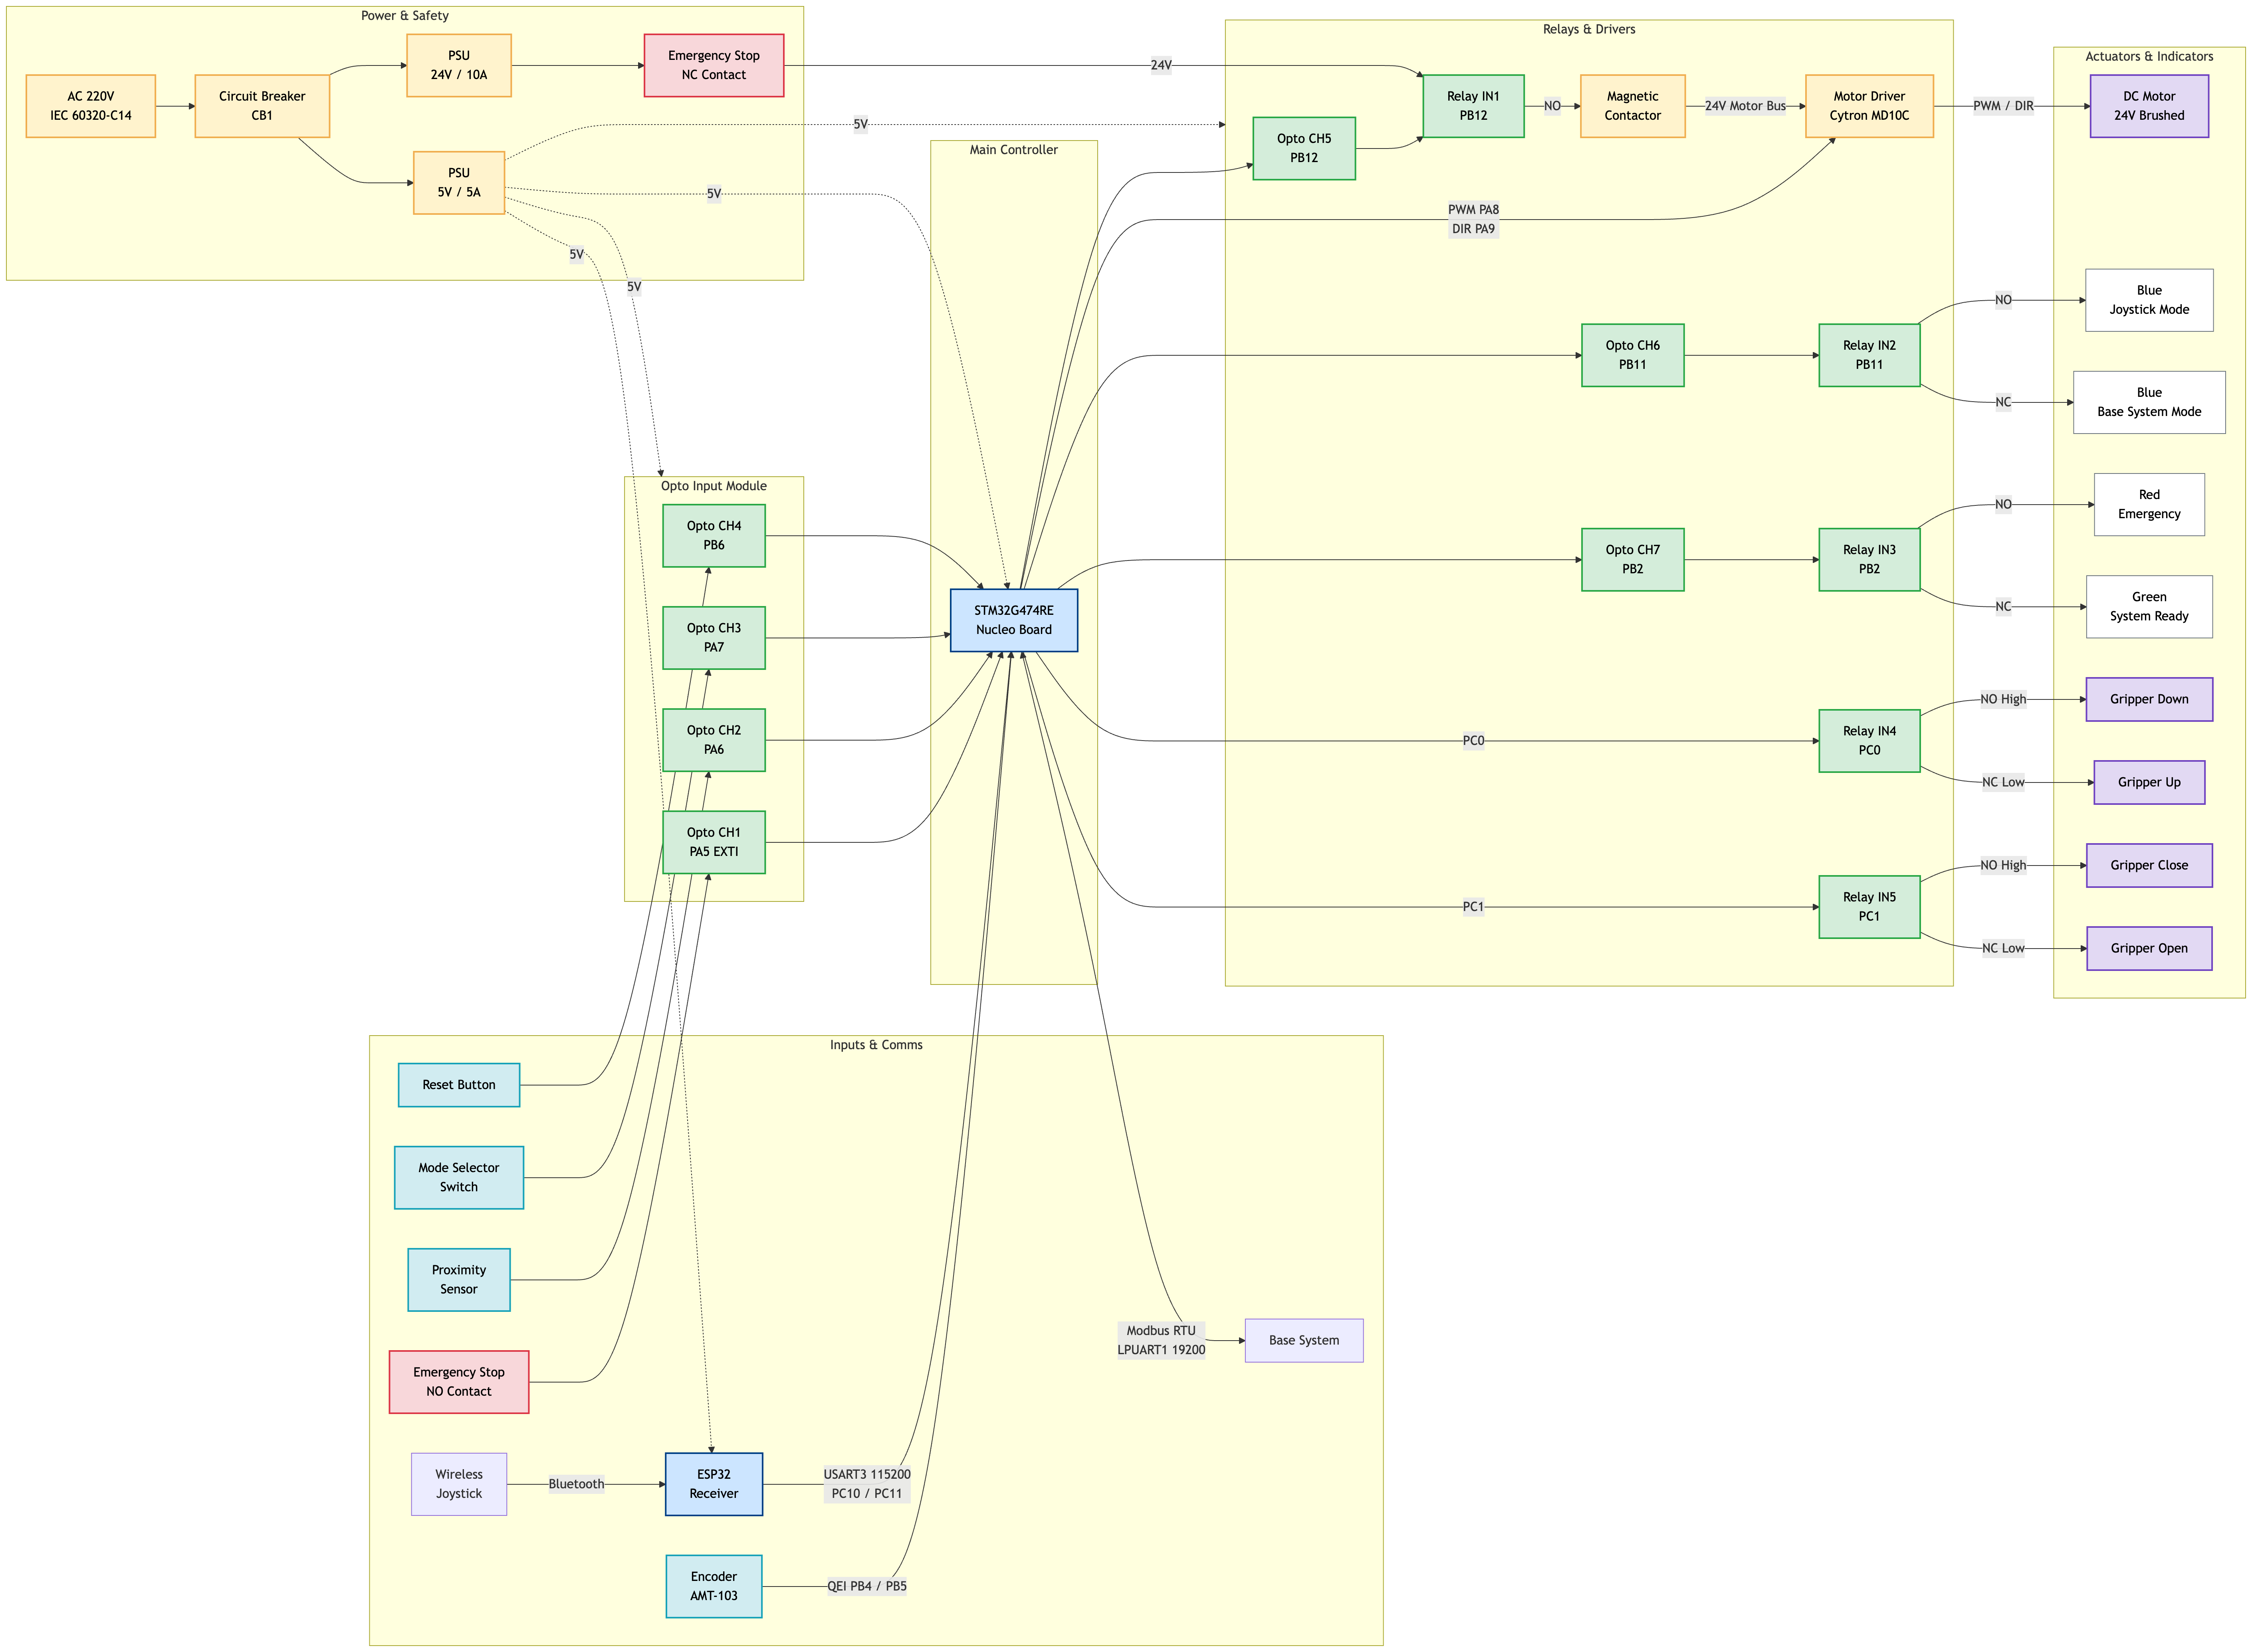
\includegraphics[width=0.95\textwidth]{images/electric_block.png}
  \caption{Electrical Block Diagram แสดงการแจกจ่ายกำลังไฟฟ้า
           และการเชื่อมต่อ Signal ของระบบ}
  \label{fig:elec_block}
\end{figure}

% ============================================================
\subsubsection{Schematic ตู้ควบคุม}
% ============================================================

Schematic ออกแบบด้วย KiCad 9.0.0 ดังแสดงใน\cref{fig:schematic}
ประกอบด้วยส่วนประกอบหลัก ได้แก่
STM32G474RE Nucleo Board เป็น Main Controller,
ESP32-DEVKITC-32UE สำหรับรับสัญญาณ Joystick ผ่าน Bluetooth,
Optocoupler Module 8 ช่อง, Relay Module 8 ช่อง,
Magnetic Contactor, PSU 24\,V/10\,A และ PSU 5\,V/5\,A

\begin{figure}[H]
  \centering
  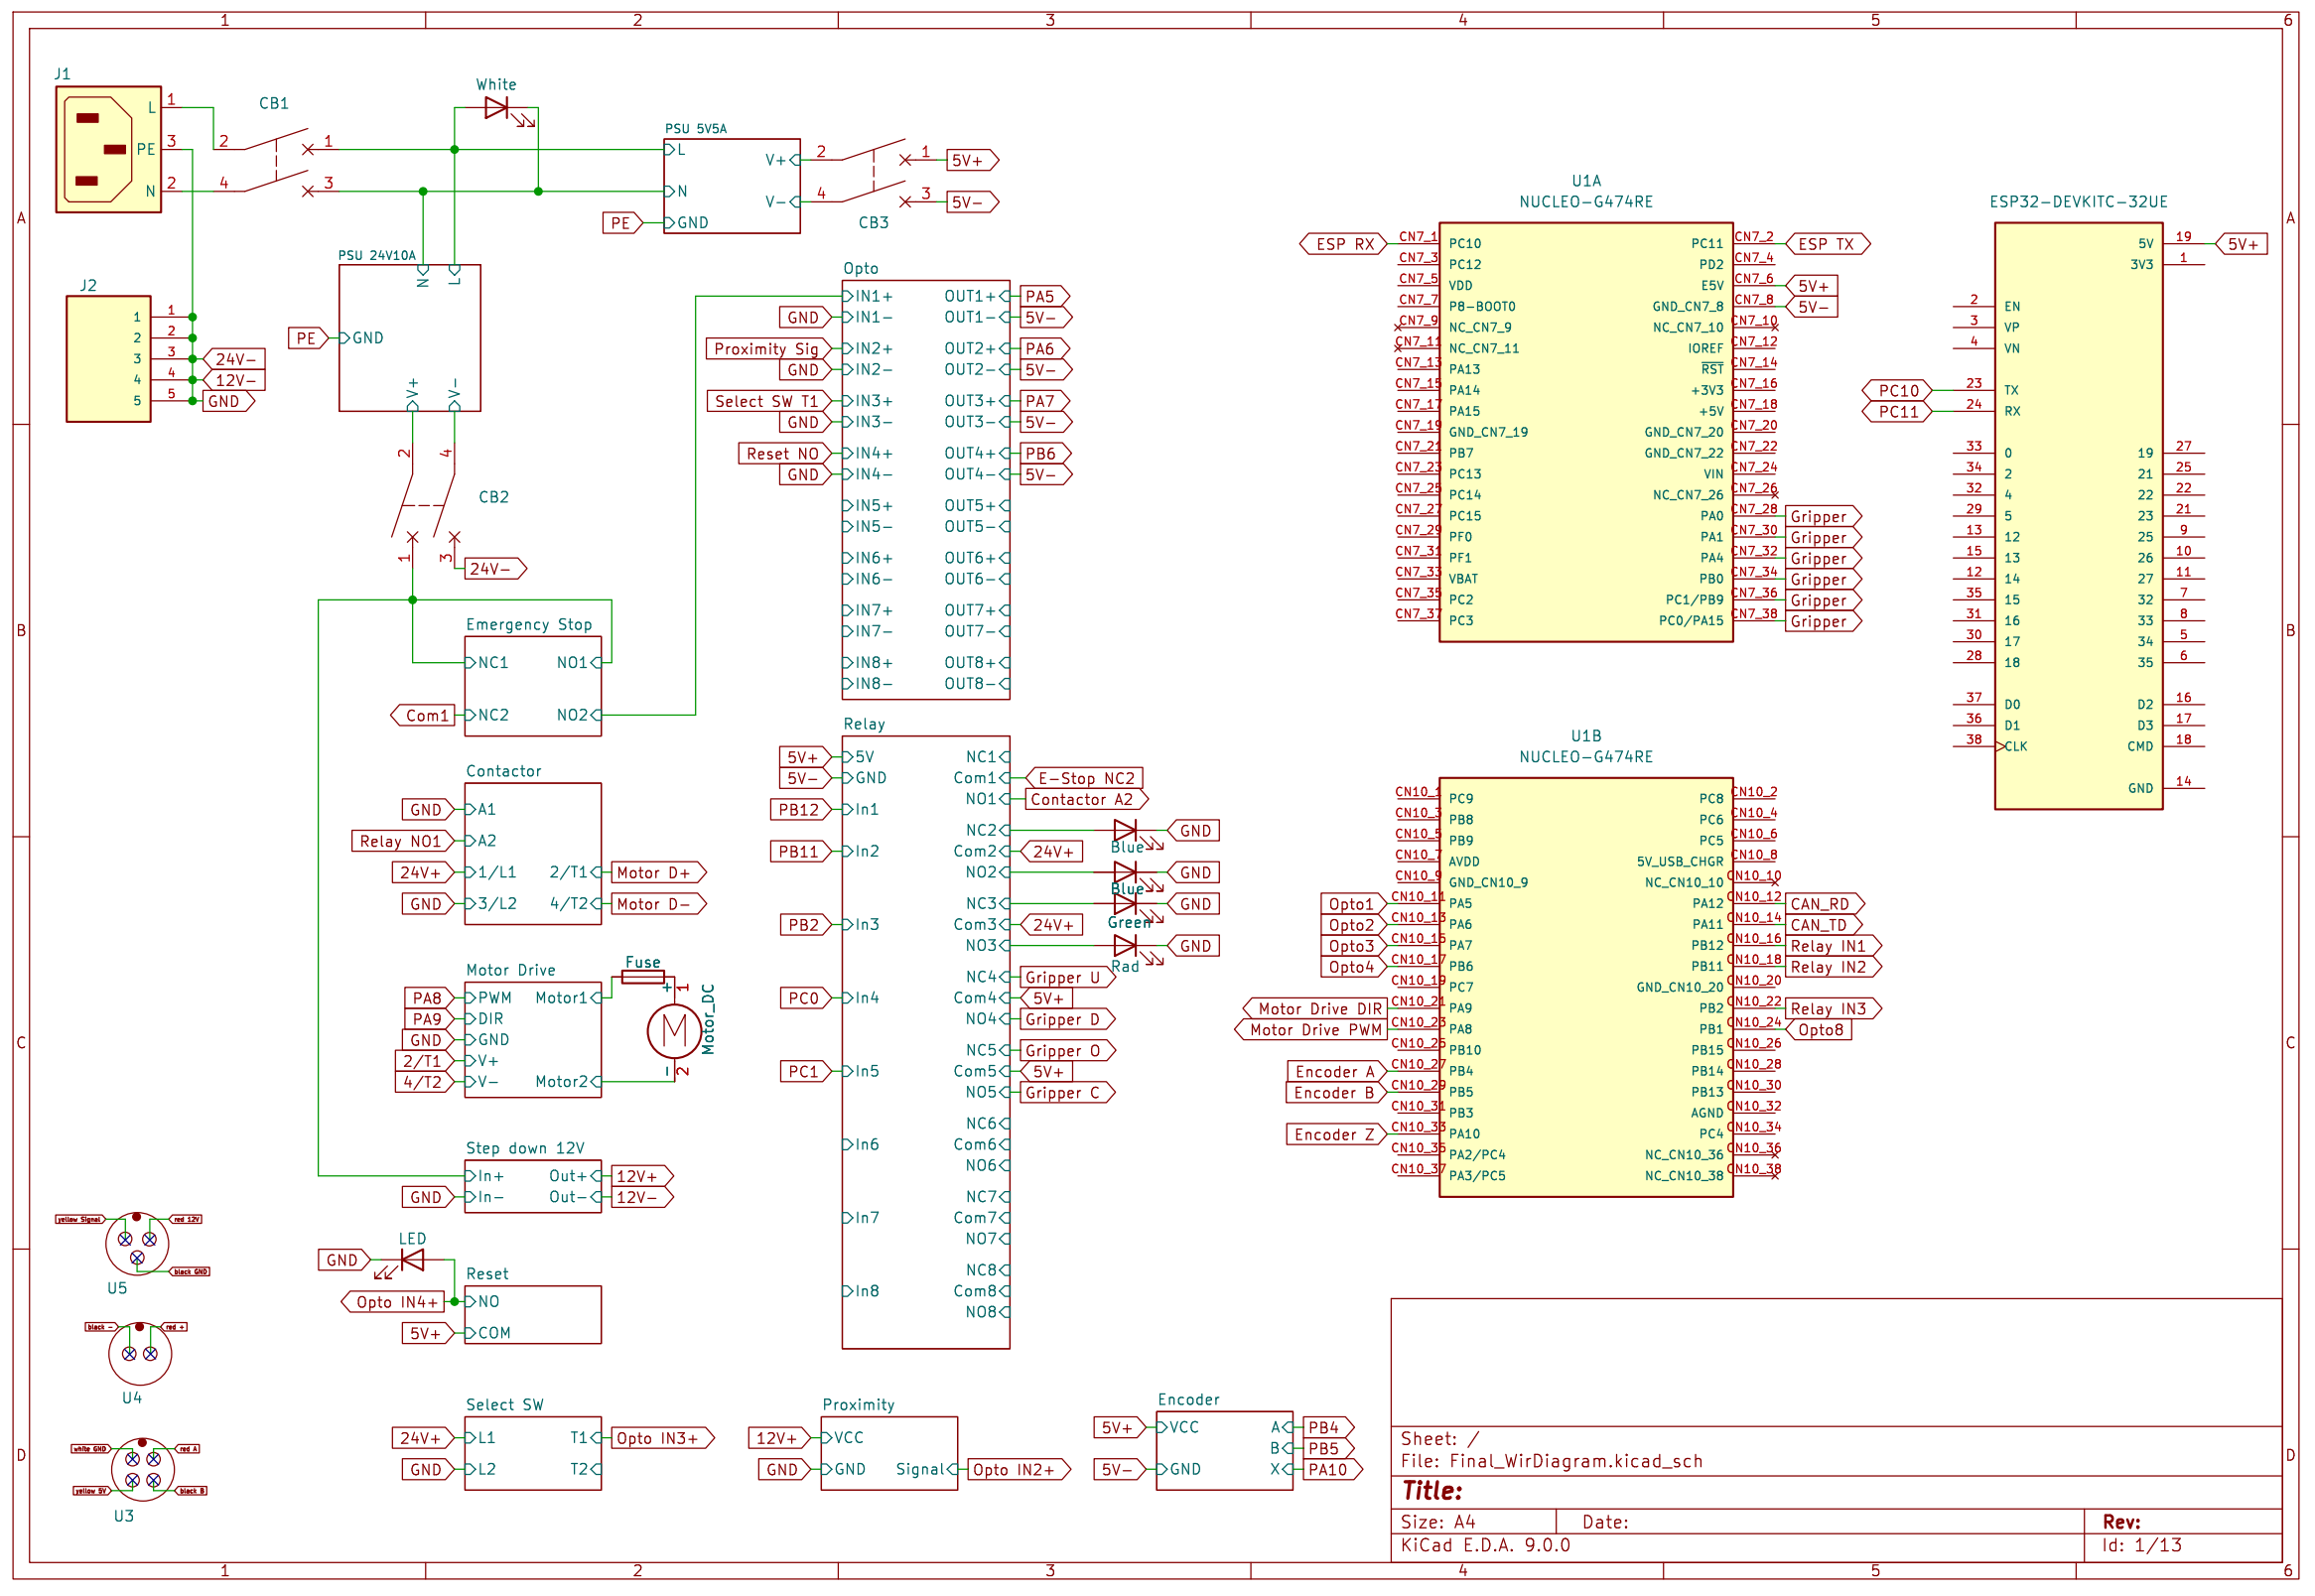
\includegraphics[width=0.95\textwidth]{images/electrical_schematic.png}
  \caption{Electrical Schematic ของตู้ควบคุมทั้งระบบ ออกแบบด้วย KiCad 9.0.0}
  \label{fig:schematic}
\end{figure}

\subsubsection{การออกแบบ PCB (PCB Design)}

PCB ออกแบบด้วย KiCad 9.0.0 เพื่อรวม STM32G474RE Nucleo Board,
ESP32-DEVKITC-32UE, Optocoupler Module, Relay Module,
Encoder Connector และ Motor Driver Connector ไว้บน Board เดียวกัน
เพื่อลดจำนวนสายเชื่อมต่อภายในตู้ควบคุมและเพิ่มความเป็นระเบียบ

\begin{figure}[H]
  \centering
  \begin{subfigure}[b]{0.48\textwidth}
    \centering
    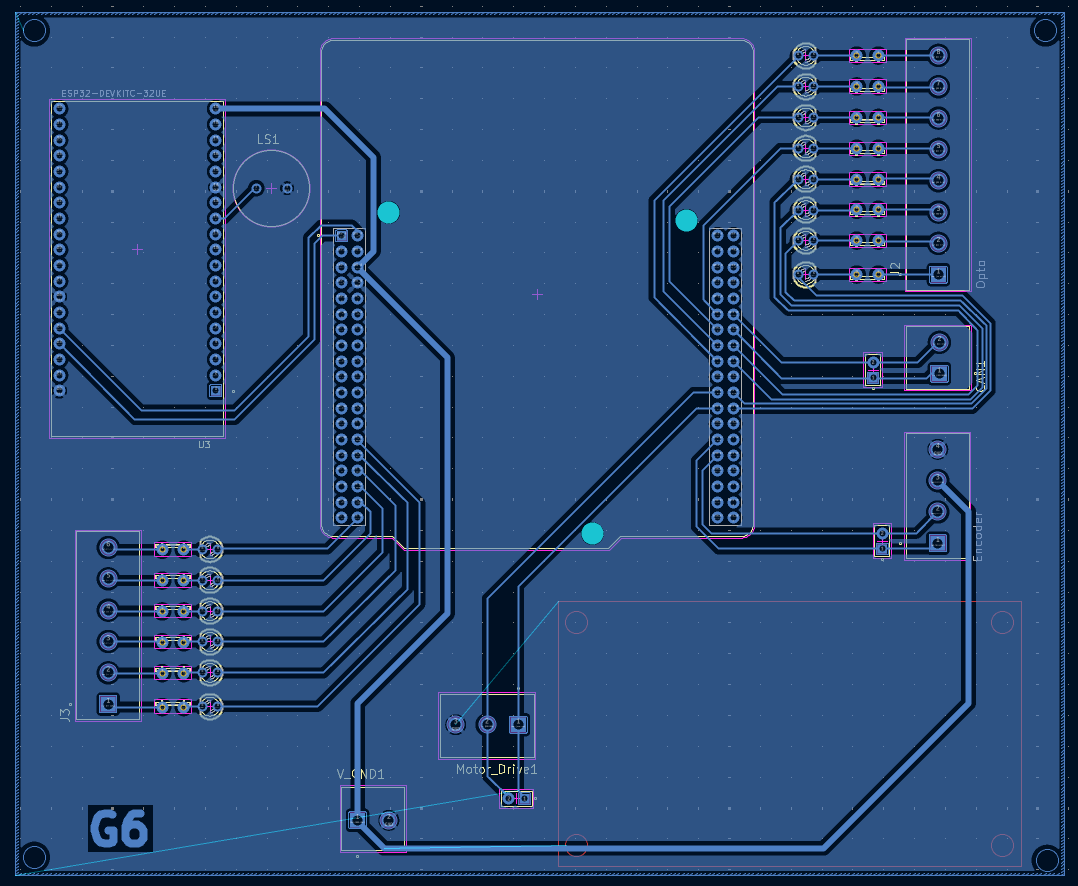
\includegraphics[width=\textwidth]{images/pcb_layout.png}
    \caption{PCB Layout (KiCad PCB Editor)}
    \label{fig:pcb_layout}
  \end{subfigure}
  \hfill
  \begin{subfigure}[b]{0.48\textwidth}
    \centering
    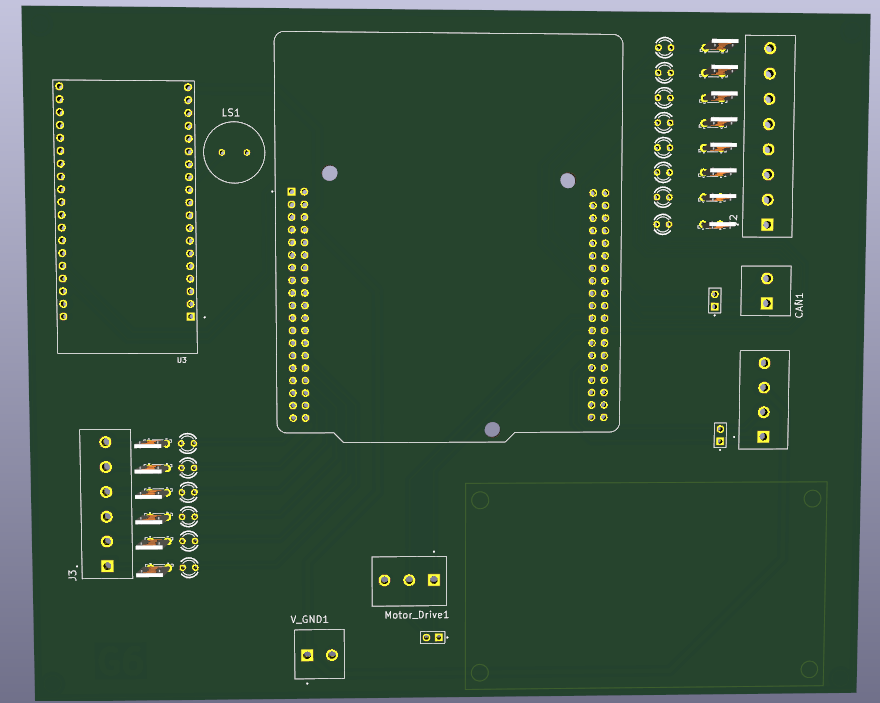
\includegraphics[width=\textwidth]{images/pcb_3d.png}
    \caption{PCB 3D Render}
    \label{fig:pcb_3d}
  \end{subfigure}
  \caption{การออกแบบ PCB สำหรับระบบควบคุม}
  \label{fig:pcb_design}
\end{figure}

% ============================================================
\subsubsection{การออกแบบวงจรป้องกัน (Protection Circuit)}
% ============================================================

ระบบมีวงจรป้องกันหลายชั้นตามข้อกำหนด E7 ดังนี้

\textbf{การป้องกัน Overcurrent:}
Circuit Breaker CB1 ทำหน้าที่ป้องกันกระแสเกินพิกัด
ในวงจร AC Input และ CB2 ป้องกันวงจร 24\,V
นอกจากนี้ Cytron MD10C มีวงจรป้องกัน Overcurrent ในตัว
และ Firmware ของ STM32 ตรวจสอบกระแสจาก Current Sensor
ทุก Control Cycle หากเกิน Threshold จะสั่งตัด PWM ทันที

\textbf{การป้องกัน Surge และ Noise:}
Optocoupler Module แยก Ground ระหว่าง High Power Side
และ Logic Side ป้องกัน Surge จากมอเตอร์ไม่ให้ทำลาย STM32
Fuse ต่ออนุกรมในวงจร Motor Driver
เพื่อป้องกันความเสียหายเมื่อเกิด Short Circuit

\textbf{Emergency Stop Hardware Interlock:}
E-Stop ทำงานในระดับ Hardware โดยตรง
ไม่ผ่าน Firmware ทำให้ไม่สามารถ Override ได้แม้ Software ค้าง
NC Contact ของปุ่ม E-Stop ต่ออยู่ใน Series กับ Coil ของ Contactor
เมื่อกด E-Stop หรือสายหลุด Contactor จะ De-energize ทันที
(Fail-Safe Design)

% ============================================================
\subsubsection{การออกแบบวงจร Optocoupler และ Relay}
% ============================================================

Optocoupler Module ทำหน้าที่แปลงสัญญาณระหว่าง
High Voltage Side (24\,V) และ Logic Side (3.3\,V/5\,V ของ STM32)
ใน 2 ทิศทาง ดังแสดงในตารางที่~\ref{tab:opto_mapping}

\begin{table}[H]
  \centering
  \caption{Optocoupler Module Channel Mapping}
  \label{tab:opto_mapping}
  \begin{tabular}{cclll}
    \toprule
    Channel & ทิศทาง & สัญญาณ & STM32 Pin & Mode \\
    \midrule
    CH1 & Input  & Emergency Stop      & PA5  & EXTI Interrupt \\
    CH2 & Input  & Proximity Sensor    & PA6  & GPIO Input \\
    CH3 & Input  & Mode Selector SW    & PA7  & GPIO Input \\
    CH4 & Input  & Reset Button        & PB6  & GPIO Input \\
    CH5 & Output & Relay IN1 (Motor)   & PB12 & GPIO Output \\
    CH6 & Output & Relay IN2 (Mode Lamp) & PB11 & GPIO Output \\
    CH7 & Output & Relay IN3 (Status Lamp) & PB2 & GPIO Output \\
    CH8 & Output & ยังไม่กำหนด        & PB1  & GPIO Output \\
    \bottomrule
  \end{tabular}
\end{table}

Relay Module รับคำสั่งจาก STM32 ผ่าน Optocoupler
และควบคุมอุปกรณ์กำลังสูงดังแสดงในตารางที่~\ref{tab:relay_mapping}

\begin{table}[H]
  \centering
  \caption{Relay Module Channel Mapping}
  \label{tab:relay_mapping}
  \begin{tabular}{cclll}
    \toprule
    Relay & STM32 Pin & COM & NO & NC \\
    \midrule
    IN1 & PB12 & 24\,V (E-Stop NC2) & Contactor A1       & --                  \\
    IN2 & PB11 & 24\,V PSU          & Pilot Blue Joystick & Pilot Blue Base     \\
    IN3 & PB2  & 24\,V PSU          & Pilot Red Emergency & Pilot Green Ready   \\
    IN4 & PC0  & 5\,V PSU           & Gripper Down (High) & Gripper Up (Low)    \\
    IN5 & PC1  & 5\,V PSU           & Gripper Close (High)& Gripper Open (Low)  \\
    \bottomrule
  \end{tabular}
\end{table}

% ============================================================
\subsubsection{STM32 Pin Assignment}
% ============================================================

ตารางที่~\ref{tab:pin_assignment} สรุป Pin Assignment ทั้งหมด
ของ STM32G474RE แบ่งตาม Subsystem

\begin{table}[H]
  \centering
  \caption{STM32G474RE Pin Assignment ของระบบ}
  \label{tab:pin_assignment}
  \begin{tabular}{lllll}
    \toprule
    Pin & Function & Mode & เชื่อมต่อกับ \\
    \midrule
    \multicolumn{4}{l}{\textit{Motor Control}} \\
    PA8 & PWM Output & TIM1 CH1         & Motor Driver PWM \\
    PA9 & DIR Output & GPIO Push-Pull    & Motor Driver DIR \\
    \midrule
    \multicolumn{4}{l}{\textit{Encoder}} \\
    PB4 & Encoder A  & TIM3 CH1 (QEI)   & AMT-103 CH A \\
    PB5 & Encoder B  & TIM3 CH2 (QEI)   & AMT-103 CH B \\
    PA10& Encoder Z  & TIM3 CH3         & AMT-103 Index \\
    \midrule
    \multicolumn{4}{l}{\textit{Communication}} \\
    PC10& UART TX    & USART3 TX        & ESP32 RX (Joystick) \\
    PC11& UART RX    & USART3 RX        & ESP32 TX (Joystick) \\
    PA11& CAN RD     & CAN1\_RD         & CAN Bus \\
    PA12& CAN TD     & CAN1\_TD         & CAN Bus \\
    \midrule
    \multicolumn{4}{l}{\textit{Safety Input (via Optocoupler)}} \\
    PA5 & E-Stop     & EXTI Interrupt   & Opto CH1 \\
    PA6 & Proximity  & GPIO Input       & Opto CH2 \\
    PA7 & Mode SW    & GPIO Input       & Opto CH3 \\
    PB6 & Reset      & GPIO Input       & Opto CH4 \\
    \midrule
    \multicolumn{4}{l}{\textit{Relay Output (via Optocoupler)}} \\
    PB12& Relay IN1  & GPIO Output      & Motor Power Control \\
    PB11& Relay IN2  & GPIO Output      & Mode Pilot Lamp \\
    PB2 & Relay IN3  & GPIO Output      & Status Pilot Lamp \\
    \midrule
    \multicolumn{4}{l}{\textit{Gripper และ Reed Switch}} \\
    PC0 & Gripper UD & GPIO Output      & Relay IN4 (Up/Down) \\
    PC1 & Gripper CO & GPIO Output      & Relay IN5 (Close/Open) \\
    PB0 & Reed Up    & GPIO Output      & Reed SW Up \\
    PA4 & Reed Down  & GPIO Output      & Reed SW Down \\
    PA1 & Reed Close & GPIO Output      & Reed SW Close \\
    PA0 & Reed Open  & GPIO Output      & Reed SW Open \\
    \bottomrule
  \end{tabular}
\end{table}

% [ใส่รูปถ่ายตู้ควบคุมที่เดินสายแล้ว]
\begin{figure}[H]
  \centering
  % [ใส่ภาพถ่ายการเดินสายจริงในตู้ควบคุม]
  \caption{ผลการเดินสายภายในตู้ควบคุมไฟฟ้า}
  \label{fig:cabinet_wiring}
\end{figure}

% ============================================================
\subsubsection{การออกแบบระบบ Joystick}
% ============================================================

ระบบ Joystick ใช้ ESP32-DEVKITC-32UE เป็น Wireless Receiver
รับสัญญาณจาก Joystick ผ่าน Bluetooth แล้วส่งต่อไปยัง STM32
ผ่าน USART3 ที่ Baud Rate 115200\,bps 8N1
ตาม Pin PC10 (TX) และ PC11 (RX)

โปรโตคอลการสื่อสารระหว่าง ESP32 และ STM32
ใช้ Data Packet ที่มีโครงสร้างคงที่
STM32 ถอดรหัส Packet และตรวจสอบ Checksum
ก่อนส่งคำสั่งไปยัง Command Parser ใน Firmware

การ Map ปุ่ม Joystick กับคำสั่งระบบแสดงในตารางที่~\ref{tab:joystick_map}

\begin{table}[H]
  \centering
  \caption{การ Map ปุ่ม Joystick กับคำสั่งระบบ}
  \label{tab:joystick_map}
  \begin{tabular}{lll}
    \toprule
    ปุ่ม Joystick & คำสั่งระบบ & หมายเหตุ \\
    \midrule
    Analog Stick (หมุนซ้าย)  & หมุนแขนซ้าย (Fine/Point) & โหมด Manual เท่านั้น \\
    Analog Stick (หมุนขวา)  & หมุนแขนขวา (Fine/Point) & โหมด Manual เท่านั้น \\
    Button: Home            & Go to Home Position      & ทุกโหมด \\
    Button: Start           & Start Auto Sequence      & โหมด Auto เท่านั้น \\
    Button: E-Stop          & Emergency Stop           & ทุกโหมด \\
    Button: Pick            & Gripper Pick Up          & โหมด Manual เท่านั้น \\
    Button: Place           & Gripper Place Down       & โหมด Manual เท่านั้น \\
    \bottomrule
  \end{tabular}
\end{table}

การสลับโหมดระหว่าง Manual (Joystick) และ Auto (Base System)
ทำผ่าน Mode Selector Switch บนตู้ควบคุม
ซึ่งส่งสัญญาณผ่าน Opto CH3 ไปยัง STM32 PA7
เมื่ออยู่ในโหมด Auto Firmware จะ Block คำสั่งจาก Joystick ทั้งหมด
ยกเว้นคำสั่ง Emergency Stop ซึ่งทำงานได้ทุกโหมดตามข้อกำหนด J1

% ============================================================
% FILE: sections/02_design_control.tex
% PURPOSE: Control Design Section — System Modeling, System ID,
%          PID Design (Loop Shaping), S-Curve, Simulation
% Compiler: XeLaTeX
%
% รูปภาพที่ต้องเตรียม (ใส่ในโฟลเดอร์ images/):
%   motor_circuit.png        -- วงจรสมมูล Armature (วาดใน draw.io)
%   simulink_motor_model.png -- Block diagram จาก Params_Estimate.slx
%   locked_rotor_scope.png   -- Oscilloscope waveform จาก Locked Rotor Test
%   chirp_raw_filtered.png   -- Plot raw vs filtered (จาก preprocess code)
%   cross_validation.png     -- Measured vs Simulated (จาก validate_parameters.m)
%   cross_val_bar.png        -- Bar chart Fit Score (จาก validate_parameters.m)
%   bode_plant.png           -- Bode plot ของ plant (จาก plant_analysis.m)
%   bode_openloop.png        -- Open-loop Bode หลัง design (จาก loop_shaping_design.m)
%   simulink_cascade.png     -- Block diagram cascade PID (screenshot Simulink)
%   scurve_360.png           -- S-curve profile 360° (จาก compute_scurve_v2.m)
%   sim_result.png           -- Simulation result 6 subplots (จาก simulate_cascade_pid_v3.m)
%   sim_current.png          -- Motor current + clamp zone
% ============================================================

% ============================================================
\subsection{การออกแบบระบบควบคุม (Control Design)}
% ============================================================

% ------------------------------------------------------------
\subsubsection{การสร้างแบบจำลองระบบ (System Modeling)}
% ------------------------------------------------------------

\paragraph{แบบจำลองมอเตอร์กระแสตรง}

ระบบขับเคลื่อนประกอบด้วยมอเตอร์กระแสตรงแบบ Brushed DC Motor
ที่ต่อกับชุดทดรอบแบบ 2 ชั้น ได้แก่ Planetary Gearbox และ Belt Drive
จากนั้นส่งกำลังไปยัง Arm ของหุ่นยนต์ การสร้างแบบจำลองแบ่งออกเป็น
2 ส่วน คือ วงจรไฟฟ้า (Electrical Subsystem) และระบบกล (Mechanical Subsystem)

\paragraph{วงจรไฟฟ้า (Electrical Subsystem)}

วงจรสมมูลของ Armature มอเตอร์กระแสตรงประกอบด้วย
ความต้านทาน $R_a$ ความเหนี่ยวนำ $L_a$ และแรงดันย้อนกลับ (Back-EMF) $e_b$
ดังแสดงใน\cref{fig:motor_circuit} โดยประยุกต์ใช้ Kirchhoff's Voltage Law (KVL)
รอบวงจร Armature ได้สมการ

\begin{equation}
  v_{in}(t) = R_a\, i_a(t) + L_a\, \frac{di_a(t)}{dt} + e_b(t)
  \label{eq:kvl}
\end{equation}

โดยที่ $v_{in}$ คือแรงดันไฟฟ้าอินพุต (V), $i_a$ คือกระแส Armature (A),
$R_a$ คือความต้านทาน Armature ($\Omega$), $L_a$ คือความเหนี่ยวนำ Armature (H)
และ $e_b$ คือแรงดันย้อนกลับ (V)

\begin{figure}[H]
  \centering
  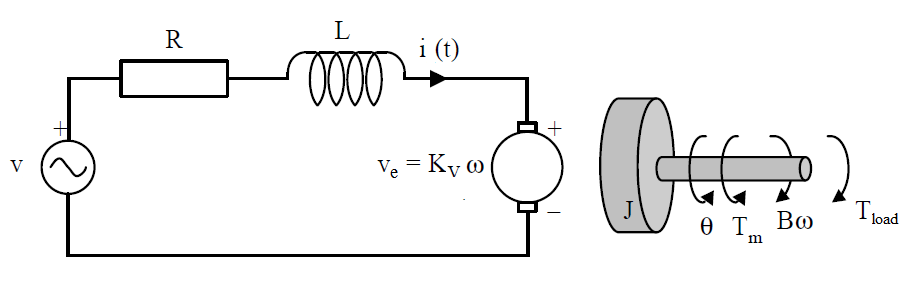
\includegraphics[width=0.65\textwidth]{images/motor_circuit.png}
  \caption{วงจรสมมูลของ Armature มอเตอร์กระแสตรง}
  \label{fig:motor_circuit}
\end{figure}

แรงดันย้อนกลับมีความสัมพันธ์กับความเร็วเชิงมุมของมอเตอร์ ($\omega_m$) ดังนี้

\begin{equation}
  e_b(t) = K_b\, \omega_m(t)
  \label{eq:bemf}
\end{equation}

โดยที่ $K_b$ คือค่าคงที่ Back-EMF (V$\cdot$s/rad)

\paragraph{ระบบกล (Mechanical Subsystem)}

แรงบิดที่มอเตอร์ผลิตได้สัมพันธ์กับกระแส Armature ดังนี้

\begin{equation}
  \tau_m(t) = K_t\, i_a(t)
  \label{eq:torque_motor}
\end{equation}

โดยที่ $K_t$ คือค่าคงที่แรงบิด (N$\cdot$m/A)

\paragraph{ชุดทดรอบ 2 ชั้น}

ระบบใช้ชุดทดรอบแบบ 2 ชั้น ได้แก่ Planetary Gearbox อัตราทดรอบ
$N_g = 24$ และ Belt Drive ที่มี Driver Pulley 24 teeth และ Driven Pulley 70 teeth
ให้อัตราทดรอบ $N_b = 70/24 = 2.917$ อัตราทดรอบรวมคือ

\begin{equation}
  N_{total} = N_g \times N_b = 24 \times \frac{70}{24} = 70
  \label{eq:gear_ratio}
\end{equation}

ความสัมพันธ์ระหว่างความเร็วเชิงมุมและแรงบิดที่ด้าน Output shaft
($\omega_{arm}$, $\tau_{out}$) กับด้าน Motor ($\omega_m$, $\tau_m$) คือ

\begin{equation}
  \omega_{arm}(t) = \frac{\omega_m(t)}{N_{total}}
  \label{eq:omega_arm}
\end{equation}

\begin{equation}
  \tau_{out}(t) = \eta\, N_{total}\, \tau_m(t)
  \label{eq:tau_out}
\end{equation}

โดยที่ $\eta$ คือประสิทธิภาพรวมของชุดทดรอบ

นำ \cref{eq:torque_motor} และ \cref{eq:tau_out} ไปใช้กับ
Newton's Second Law ที่ Output shaft

\begin{equation}
  J\, \frac{d\omega_{arm}(t)}{dt} = \tau_{out}(t) - b\, \omega_{arm}(t)
  \label{eq:newton}
\end{equation}

\begin{equation}
  J\, \frac{d\omega_{arm}(t)}{dt} = \eta\, N_{total}\, K_t\, i_a(t) - b\, \omega_{arm}(t)
  \label{eq:newton_expand}
\end{equation}

โดยที่ $J$ คือโมเมนต์ความเฉื่อยรวมของ Arm, Gripper และ Connection Rod
(kg$\cdot$m$^2$) และ $b$ คือสัมประสิทธิ์การหน่วงแบบ Viscous (N$\cdot$m$\cdot$s/rad)

\paragraph{Block Diagram ของระบบ}

Block Diagram ของแบบจำลองระบบมอเตอร์ที่สร้างใน Simulink
แสดงดัง\cref{fig:motor_block} ซึ่งประกอบด้วย Electrical Loop
ที่ป้อนกลับด้วย Back-EMF และ Mechanical Loop
ที่ป้อนกลับด้วย Viscous Damping

\begin{figure}[H]
  \centering
  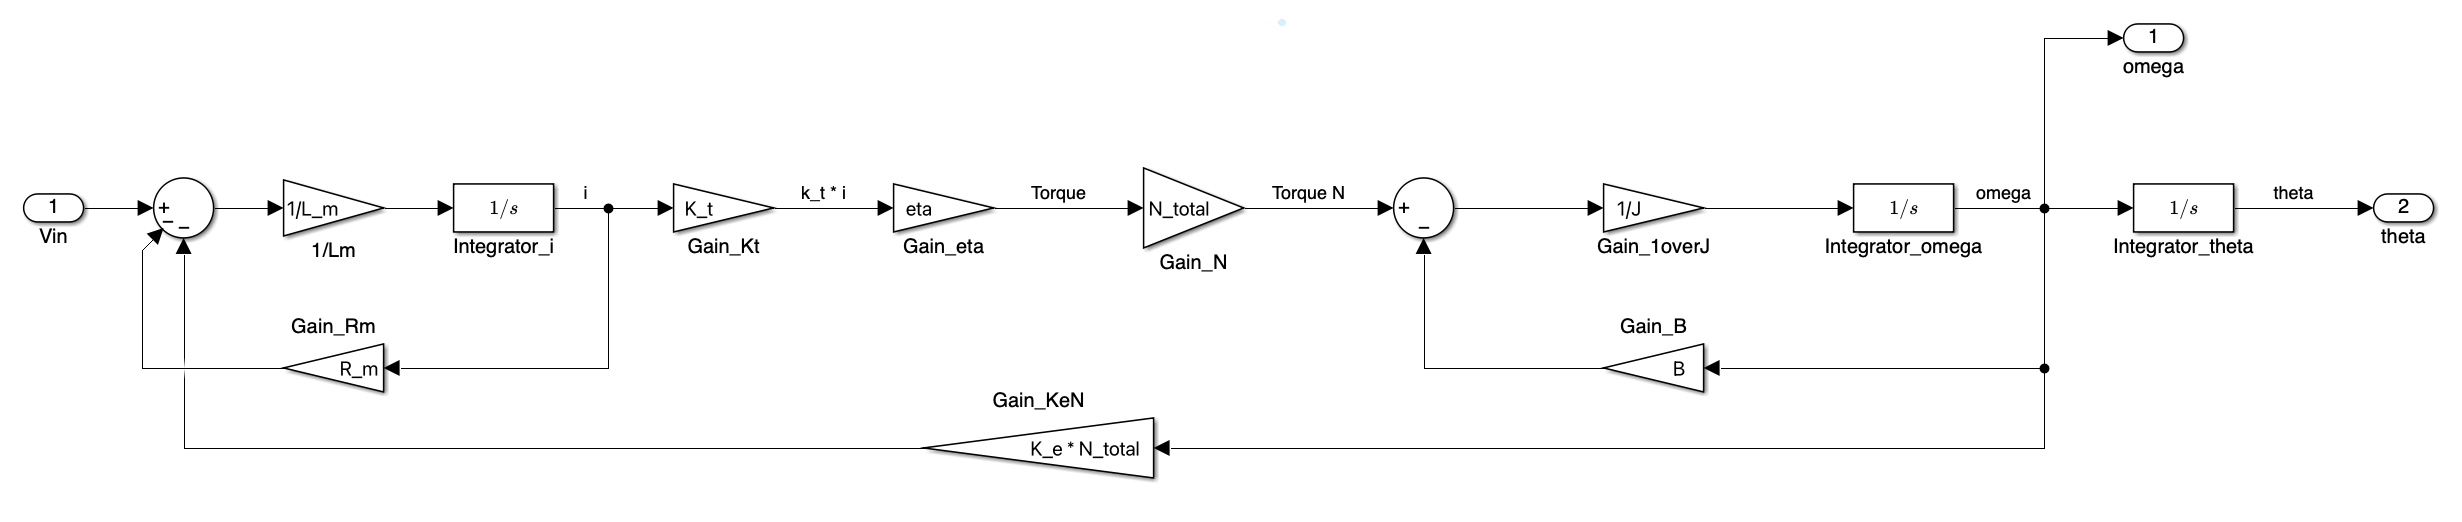
\includegraphics[width=0.92\textwidth]{images/simulink_motor_model.png}
  \caption{Block Diagram ของระบบมอเตอร์กระแสตรงพร้อมชุดทดรอบใน Simulink}
  \label{fig:motor_block}
\end{figure}

\paragraph{Transfer Function}

แปลง \cref{eq:kvl,eq:bemf,eq:newton_expand} เป็น Laplace domain
โดยสมมติเงื่อนไขเริ่มต้นเป็นศูนย์

\begin{align}
  V_{in}(s) &= (R_a + L_a s)\, I_a(s) + K_b\, N_{total}\, \Omega_{arm}(s)
  \label{eq:lap_elec} \\
  (Js + b)\, \Omega_{arm}(s) &= \eta\, N_{total}\, K_t\, I_a(s)
  \label{eq:lap_mech}
\end{align}

จาก \cref{eq:lap_mech} แทน $I_a(s)$ ลงใน \cref{eq:lap_elec}
แล้วจัดรูปได้ Velocity Transfer Function ดังนี้

\begin{equation}
  G_{vel}(s) = \frac{\Omega_{arm}(s)}{V_{in}(s)}
             = \frac{\eta K_t N_{total} / (L_a J)}
                    {s^2 + \left(\dfrac{R_a}{L_a} + \dfrac{b}{J}\right)s
                         + \dfrac{R_a b + K_b K_t N_{total}^2}{L_a J}}
  \label{eq:Gvel}
\end{equation}

สำหรับ Position Transfer Function เพิ่ม Integrator เนื่องจาก
$\Theta_{arm}(s) = \Omega_{arm}(s)/s$

\begin{equation}
  G_{pos}(s) = \frac{\Theta_{arm}(s)}{V_{in}(s)}
             = \frac{\eta K_t N_{total} / (L_a J)}
                    {s\left[s^2 + \left(\dfrac{R_a}{L_a} + \dfrac{b}{J}\right)s
                         + \dfrac{R_a b + K_b K_t N_{total}^2}{L_a J}\right]}
  \label{eq:Gpos}
\end{equation}

แทนค่าตัวเลขจาก System Identification

\begin{align}
  K_{num} &= \frac{\eta K_t N_{total}}{L_a J}
           = \frac{0.836 \times 0.04065 \times 70}{0.001448 \times 0.728}
           = \frac{2.376}{0.001054} = 2254 \notag \\
  a_1     &= \frac{R_a}{L_a} + \frac{b}{J}
           = \frac{1.453}{0.001448} + \frac{0.193}{0.728}
           = 1003.5 + 0.265 = 1003.8 \notag \\
  a_0     &= \frac{R_a b + K_b K_t N_{total}^2}{L_a J} \notag \\
           &= \frac{(1.453)(0.193) + (0.04165)(0.04065)(70)^2}{(0.001448)(0.728)} \notag \\
           &= \frac{0.280 + 8.297}{0.001054} = 8136 \notag
\end{align}

ดังนั้น Transfer Function เชิงตัวเลขคือ

\begin{equation}
  G_{vel}(s) = \frac{2254}{s^2 + 1003.8\,s + 8136}
  \label{eq:Gvel_num}
\end{equation}

\begin{equation}
  G_{pos}(s) = \frac{2254}{s\left(s^2 + 1003.8\,s + 8136\right)}
  \label{eq:Gpos_num}
\end{equation}

% ------------------------------------------------------------
\subsubsection{การทำ System Identification}
% ------------------------------------------------------------

\paragraph{พารามิเตอร์ที่วัดโดยตรง: Locked Rotor Test}

ค่า $R_a$ และ $L_a$ วัดด้วย Locked Rotor Test โดยจ่ายแรงดัน Step
ผ่าน Shunt Resistor $R_{sh} = 0.1\,\Omega$ แล้ววัดแรงดันตกคร่อม Shunt
ด้วย Oscilloscope ดังแสดงใน\cref{fig:locked_rotor_scope}
เพื่อหาค่า $V_{max}$ และค่าคงเวลา $\tau$ แล้วคำนวณด้วยสูตร

\paragraph{การเลือกค่า $R_{sh}$}

การเลือกค่า $R_{sh} = 0.1\,\Omega$ มาจากเงื่อนไข 2 ข้อดังนี้

\textbf{เงื่อนไขที่ 1: ไม่รบกวนวงจร}
ค่า $R_{sh}$ ต้องมีขนาดเล็กเมื่อเทียบกับ $R_a$ เพื่อไม่ให้กระทบต่อพฤติกรรมของวงจร
โดยกำหนดค่าคงที่ $k = 0.1$ ดังนี้

\begin{equation}
  \frac{R_{sh}}{R_a} < k \implies R_{sh} < 0.1 \times 1.453 = 0.1453\,\Omega
  \label{eq:rsh_condition1}
\end{equation}

\textbf{เงื่อนไขที่ 2: ทนกำลังไฟได้}
ประมาณกระแส Stall จากแรงดันสูงสุดและค่า $R_a$ ที่วัดได้

\begin{equation}
  I_{stall} \approx \frac{V_{in}}{R_a} = \frac{24}{1.453} \approx 16.5\,\text{A}
  \label{eq:i_stall}
\end{equation}

กำลังที่ $R_{sh}$ ต้องทนได้คือ

\begin{equation}
  P_{sh} = I_{stall}^2 \cdot R_{sh} = (16.5)^2 \times 0.1 \approx 27.2\,\text{W}
  \label{eq:p_sh}
\end{equation}

จากทั้งสองเงื่อนไข จึงเลือก $R_{sh} = 0.1\,\Omega$ 
ซึ่งน้อยกว่าขีดจำกัด $0.1453\,\Omega$ และต้องใช้ตัวต้านทานที่ทนกำลังได้อย่างน้อย $30\,\text{W}$

\paragraph{ที่มาของสูตร}

ขณะ Locked Rotor แกนมอเตอร์หยุดนิ่ง ทำให้ $\omega_m = 0$ 
และ Back-EMF หายไป $e_b = K_b\,\omega_m = 0$ วงจรจึงเหลือเพียง

\begin{equation}
  V_{in} = (R_a + R_{sh})\,i(t) + L_a\,\frac{di(t)}{dt}
  \label{eq:locked_rotor_circuit}
\end{equation}

\textbf{การหา $R_a$:}
ที่ Steady State กระแสนิ่ง $\frac{di}{dt} = 0$ และวัด $V_{sh,ss}$ ได้จาก Oscilloscope
ดังนั้น $i_{ss} = V_{sh,ss}/R_{sh}$ แทนกลับได้

\begin{equation}
  R_a = R_{sh}\left(\frac{V_{in}}{V_{sh,ss}} - 1\right)
  \label{eq:Ra_derive}
\end{equation}

\textbf{การหา $L_a$:}
Solution ของวงจร RL คือ $i(t) = i_{ss}(1 - e^{-t/\tau})$ 
โดยที่ $\tau = L_a/(R_a + R_{sh})$ จัดรูปได้

\begin{equation}
  L_a = \tau\,(R_a + R_{sh}) = R_{sh}\left(\tau\,\frac{V_{in}}{V_{sh,ss}}\right)
  \label{eq:La_derive}
\end{equation}

\begin{equation}
  R_a = R_{sh}\left(\frac{V_{in}}{V_{sh}} - 1\right), \qquad
  L_a = R_{sh}\left(\tau\,\frac{V_{in}}{V_{sh}}\right)
  \label{eq:locked_rotor}
\end{equation}

โดยที่ $V_{sh}$ คือแรงดันตกคร่อม Shunt ที่ Steady State

\begin{figure}[H]
  \centering
  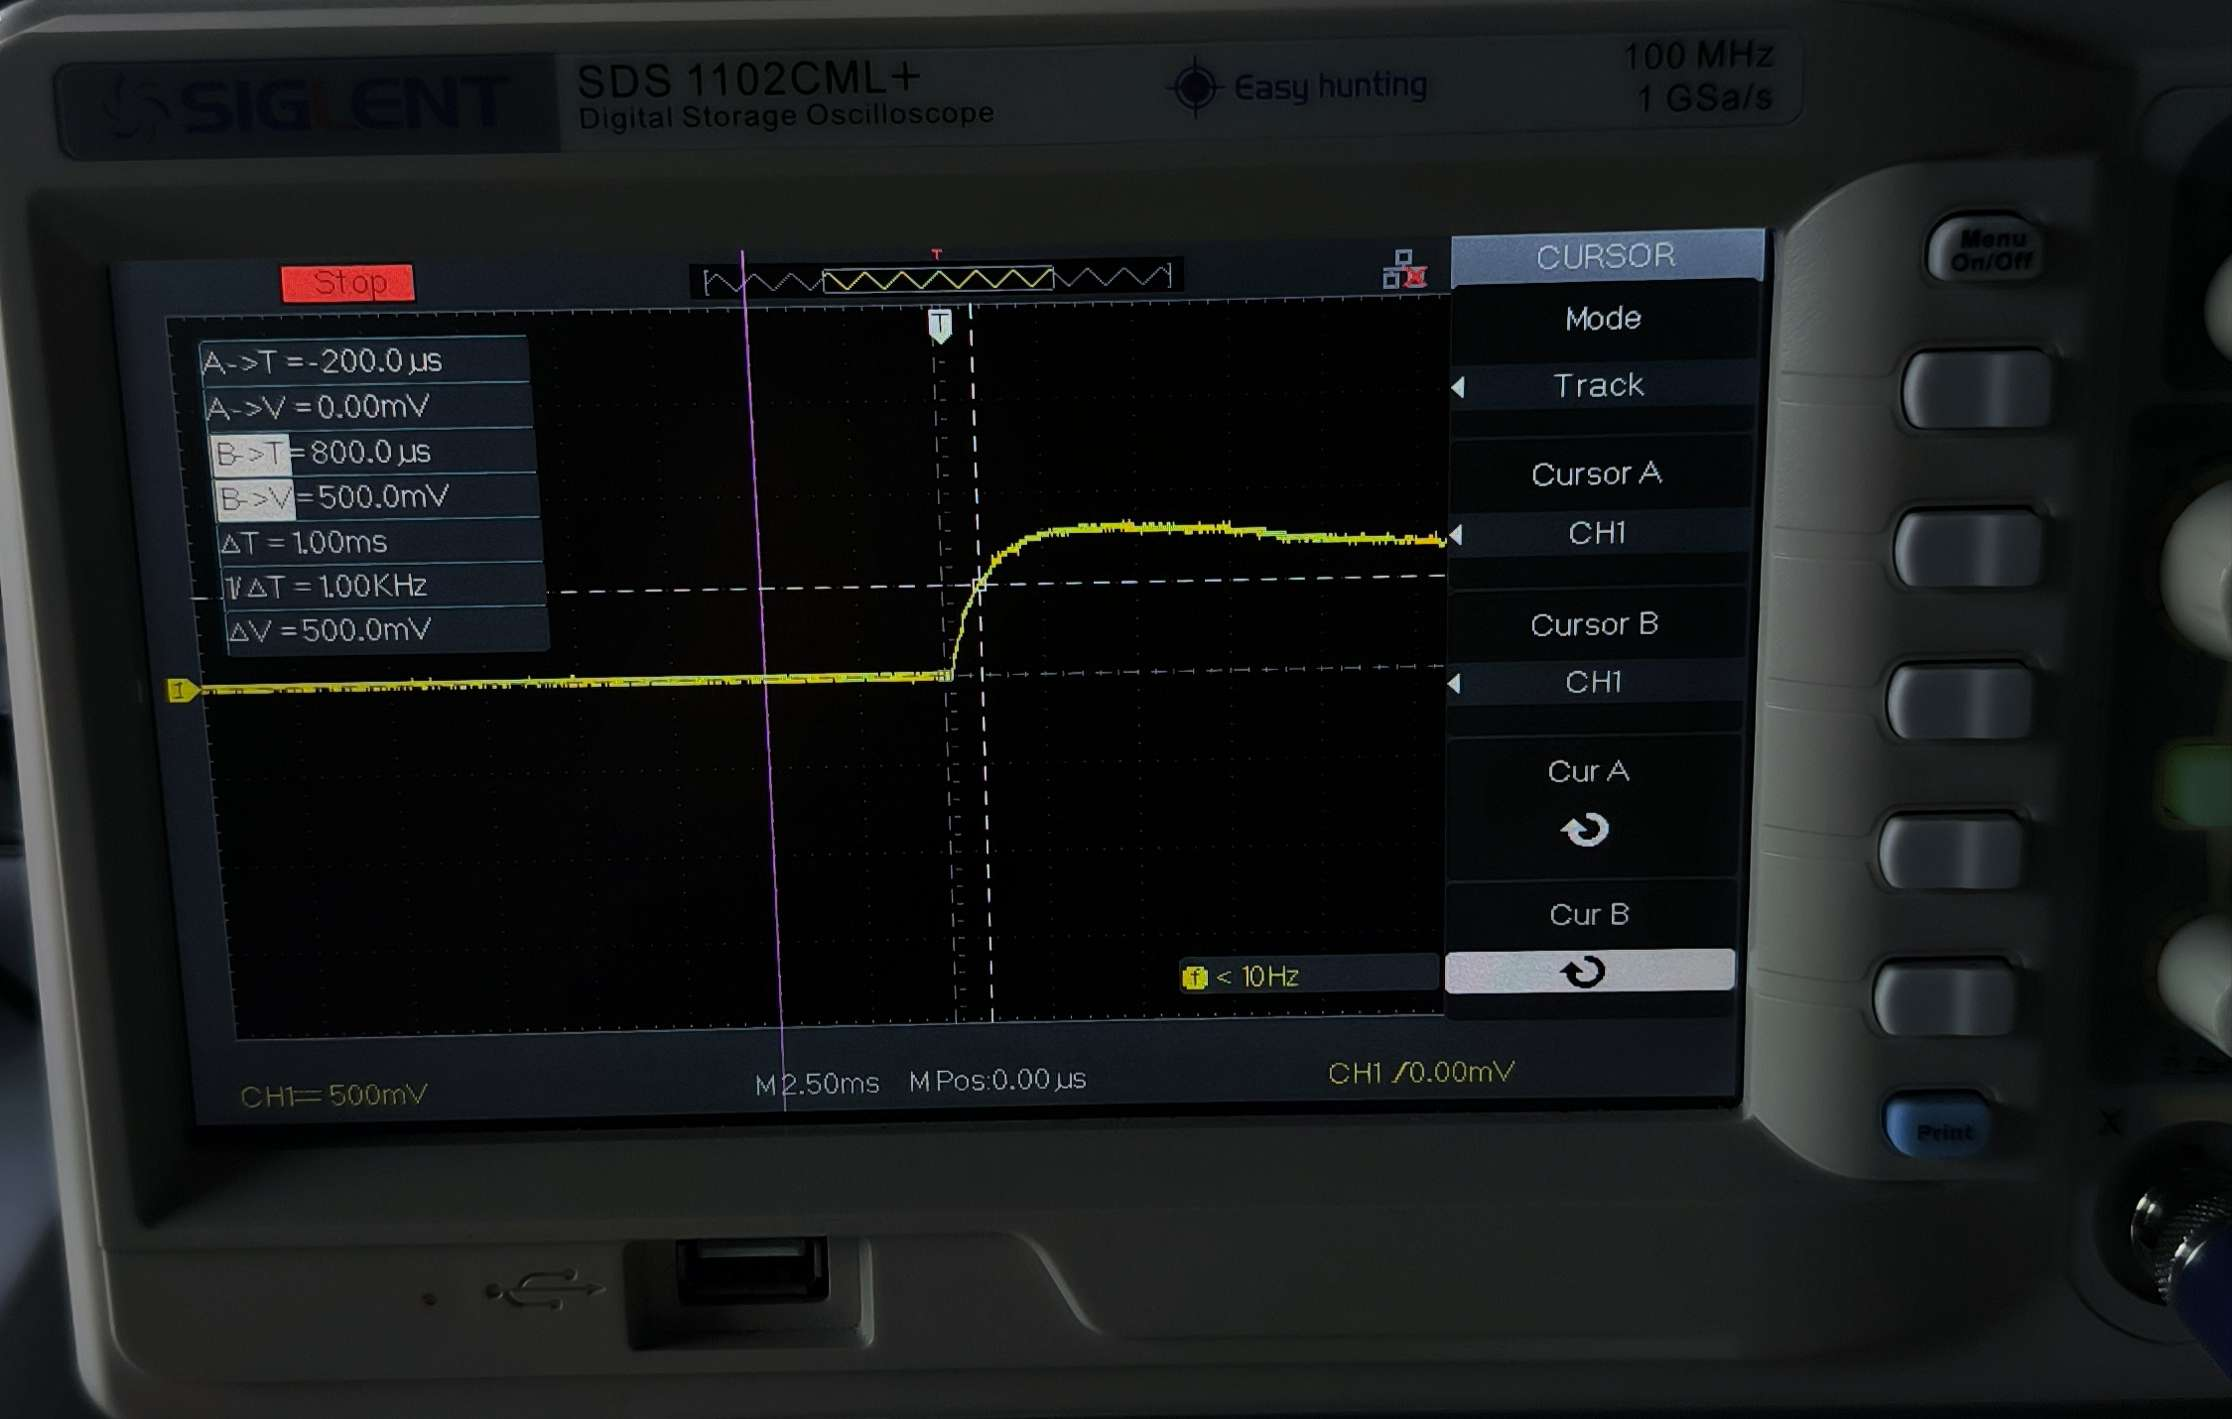
\includegraphics[width=0.70\textwidth]{images/locked_rotor_scope.png}
  \caption{Oscilloscope Waveform จาก Locked Rotor Test แสดง $V_{max}$ และ $\tau$}
  \label{fig:locked_rotor_scope}
\end{figure}

\paragraph{การเลือกแรงดันทดสอบ}

ทดสอบที่แรงดัน 3 ระดับ ได้แก่ $V_{in} = 6$, $9$ และ $12$\,V 
เพื่อตรวจสอบความสม่ำเสมอของค่าที่วัดได้ในแต่ละระดับ
ผลสรุปแสดงในตารางที่~\ref{tab:locked_rotor_all}

\begin{table}[H]
  \centering
  \caption{เปรียบเทียบผลการวัด $R_a$ และ $L_a$ จาก Locked Rotor Test ทั้ง 3 แรงดัน}
  \label{tab:locked_rotor_all}
  \begin{tabular}{ccccc}
    \toprule
    $V_{in}$ (V) & $\bar{R}_a$ ($\Omega$) & $\sigma_{R_a}$ ($\Omega$) 
                 & $\bar{L}_a$ (H)        & $\sigma_{L_a}$ (H) \\
    \midrule
    6  & 1.7300 & 0.0374 & 0.001490 & 0.000062 \\
    9  & 1.5398 & 0.0604 & 0.001473 & 0.000095 \\
    12 & 1.4534 & 0.0523 & 0.001448 & 0.000055 \\
    \bottomrule
  \end{tabular}
\end{table}

จากตารางพบว่าค่า $R_a$ มีแนวโน้มลดลงเมื่อแรงดันเพิ่มขึ้น 
ซึ่งเป็นผลจากสองปัจจัยหลัก ได้แก่
\begin{itemize}
  \item \textbf{Contact Resistance:} ที่แรงดันต่ำ กระแสที่ไหลผ่านน้อย
        ทำให้ความต้านทานสัมผัสของ Brush และขั้วต่อมีนัยสำคัญมากขึ้น
        เมื่อแรงดันสูงขึ้น สัดส่วนของ Contact Resistance ต่อ $R_a$ รวมลดลง
  \item \textbf{Signal-to-Noise Ratio:} ที่ $V_{in} = 6$\,V 
        แรงดันตกคร่อม Shunt $V_{sh}$ มีค่าต่ำ ทำให้ Noise 
        มีผลต่อการอ่านค่ามากกว่า ส่งผลให้ค่าที่วัดได้มี Error สูงกว่า
\end{itemize}

จึงเลือกใช้ผลจาก $V_{in} = 12$\,V เป็นค่าอ้างอิง เนื่องจากสองเหตุผล ได้แก่
\begin{enumerate}
  \item ใกล้เคียงกับแรงดันใช้งานจริง $24$\,V มากที่สุดในบรรดาแรงดันที่ทดสอบ
        ทำให้สภาวะของ Brush Contact ใกล้เคียงกับการทำงานจริงมากที่สุด
  \item ไม่ทดสอบที่ $24$\,V เนื่องจากขณะ Locked Rotor 
        กระแส Stall $I_{stall} \approx V_{in}/R_a = 24/1.453 \approx 16.5$\,A 
        จะทำให้ $R_{sh}$ รับกำลัง $P_{sh} = I_{stall}^2 \cdot R_{sh} 
        = (16.5)^2 \times 0.1 \approx 27.2$\,W ซึ่งเกินพิกัดและอาจเป็นอันตรายได้
\end{enumerate}

เลือกใช้ค่าทดสอบที่ $V_{in} = 12$\,V จำนวน 3 ครั้ง ผลการวัดแสดงใน\cref{tab:locked_rotor}

\begin{table}[H]
  \centering
  \caption{ผลการวัด $R_a$ และ $L_a$ จาก Locked Rotor Test ที่ 12\,V}
  \label{tab:locked_rotor}
  \begin{tabular}{lcccc}
    \toprule
    Run & $V_{max}$ (V) & $\tau$ (s) & $R_a$ ($\Omega$) & $L_a$ (H) \\
    \midrule
    1 & 0.740 & 0.00090 & 1.52162 & 0.001459 \\
    2 & 0.780 & 0.00090 & 1.43846 & 0.001385 \\
    3 & 0.800 & 0.00100 & 1.40000 & 0.001500 \\
    \midrule
    \textbf{Mean} & & & \textbf{1.45336} & \textbf{0.001448} \\
    \bottomrule
  \end{tabular}
\end{table}

ค่าเฉลี่ยที่ได้จากการทดสอบ 3 ครั้ง คือ $R_a = 1.453\,\Omega$ และ $L_a = 1.448\,\text{mH}$
ซึ่งจะใช้เป็นค่าอ้างอิงในการสร้างแบบจำลองและออกแบบระบบควบคุมในหัวข้อถัดไป

\paragraph{การเลือกสัญญาณ Excitation}

เลือกใช้ Chirp Signal เป็น Excitation เนื่องจากเป็นสัญญาณ Sine Wave 
ที่ความถี่เพิ่มขึ้นเรื่อย ๆ ตามเวลา (Frequency Sweep) 
ทำให้สามารถ Excite พฤติกรรมของมอเตอร์ได้ครอบคลุมทั้งย่านความถี่ต่ำ 
(Slow Dynamics เช่น Inertia และ Viscous Damping) 
และย่านความถี่สูง (Fast Dynamics เช่น Friction) ภายใน Input เดียว
สัญญาณอื่น เช่น Step หรือ Impulse มีพลังงานกระจุกตัวอยู่ที่ความถี่เดียว
จึงให้ข้อมูล Frequency Content ที่ไม่ครอบคลุมเท่า

\paragraph{การเลือกย่านความถี่ 0.1--2.0\,Hz}

ขอบล่าง $f_{min} = 0.1$\,Hz เลือกเพื่อให้ครอบคลุม Slow Dynamics 
ของระบบ โดยเฉพาะ Inertia $J$ ที่มีผลเด่นชัดที่ความถี่ต่ำมาก

ขอบบน $f_{max} = 2.0$\,Hz กำหนดจาก Mechanical Bandwidth ของระบบ
ซึ่งประมาณได้จากพารามิเตอร์ที่วัดได้ดังนี้

\begin{equation}
  f_{mech} = \frac{1}{2\pi}\sqrt{\frac{R_a b + K_b K_t N^2}{L_a J}}
           = \frac{1}{2\pi}\sqrt{8136}
           \approx 14.4\,\text{Hz}
  \label{eq:f_mech}
\end{equation}

ค่า $f_{max} = 2.0$\,Hz คิดเป็นประมาณ 14\% ของ $f_{mech}$ 
ซึ่งอยู่ในย่านที่ระบบยังตามสัญญาณได้ดี 
และไม่สูงจนมอเตอร์ไม่สามารถตอบสนองได้ทัน
นอกจากนี้ยังเลือกทดสอบ 3 กลุ่มความถี่ ได้แก่ 
0.1--0.5\,Hz, 0.1--1.0\,Hz และ 0.1--2.0\,Hz 
เพื่อตรวจสอบความสม่ำเสมอของผลการ Estimate ในแต่ละย่านความถี่

\paragraph{การ Preprocess ข้อมูล}

ข้อมูลดิบจาก Hardware กรองด้วย Butterworth Low-pass Filter Order 4
ที่ Cutoff Frequency $f_c = 10$\,Hz โดยเลือกจากเงื่อนไข

\begin{equation}
  f_c = 5 \times f_{max} = 5 \times 2.0 = 10\,\text{Hz}
  \label{eq:fc}
\end{equation}

เพื่อให้สัญญาณ Chirp ทุกความถี่ผ่านได้เต็มที่ 
ในขณะที่ลด Noise ความถี่สูงจาก Encoder และ Electrical Noise ออก
เลือก Butterworth เนื่องจากมี Flat Passband 
ไม่บิดเบือน Amplitude ของสัญญาณในย่านที่สนใจ
และ Order 4 ให้ Attenuation ที่ $10 f_c = 100$\,Hz สูงถึง

\begin{equation}
  A = -20 \times 4 \times \log_{10}\!\left(\frac{100}{10}\right) = -80\,\text{dB}
  \label{eq:attenuation}
\end{equation}

ซึ่งเพียงพอในการกำจัด Noise ความถี่สูงออกจากสัญญาณ
ใช้ \texttt{filtfilt} แทน \texttt{filter} ธรรมดา 
เพื่อให้ Phase Shift เป็นศูนย์ตลอดทุกความถี่
เนื่องจากหาก Phase Shift ไม่เป็นศูนย์ 
จะทำให้ความสัมพันธ์ระหว่าง $V_{in}$ และ $\omega_{arm}$ในเชิงเวลาคลาดเคลื่อน
ส่งผลให้ Parameter Estimator ได้ค่าพารามิเตอร์ที่ผิดพลาดได้

\textbf{ผลการตรวจสอบความถูกต้องของแบบจำลอง (Model Validation)}

การตรวจสอบความถูกต้องของแบบจำลองกระทำโดยนำแบบจำลองไปจำลองการทำงานเปรียบเทียบกับข้อมูลจริงจาก Hardware ในเงื่อนไขต่าง ๆ (Cross-Validation) เพื่อคำนวณ Fit Score และ NRMSE โดยรายละเอียดผลการตรวจสอบโดยละเอียดแสดงใน\cref{subsec:model_validation_results}

\begin{table}[H]
  \centering
  \caption{พารามิเตอร์ที่ได้จาก System Identification}
  \label{tab:sysid_params}
  \begin{tabular}{llccc}
    \toprule
    พารามิเตอร์ & สัญลักษณ์ & ค่า & หน่วย & วิธีการ \\
    \midrule
    Armature Resistance    & $R_a$  & 1.4534   & $\Omega$              & Locked Rotor Test \\
    Armature Inductance    & $L_a$  & 0.001448 & H                     & Locked Rotor Test \\
    Back-EMF Constant      & $K_b$  & 0.04165  & V$\cdot$s/rad         & Parameter Estimation \\
    Torque Constant        & $K_t$  & 0.04065  & N$\cdot$m/A           & Parameter Estimation \\
    Viscous Damping        & $b$    & 0.19279  & N$\cdot$m$\cdot$s/rad & Parameter Estimation \\
    Moment of Inertia      & $J$    & 0.72762  & kg$\cdot$m$^2$        & Parameter Estimation \\
    Gear Ratio (Planetary) & $N_g$  & 24       & --                    & Datasheet \\
    Belt Drive Ratio       & $N_b$  & 2.917    & --                    & การออกแบบ \\
    Total Gear Ratio       & $N$    & 70       & --                    & $N_g \times N_b$ \\
    Efficiency             & $\eta$ & 0.836    & --                    & Parameter Estimation \\
    \bottomrule
  \end{tabular}
\end{table}

% ------------------------------------------------------------
\subsubsection{การออกแบบตัวควบคุม PID ด้วย Root Locus}
% ------------------------------------------------------------

\paragraph{โครงสร้างระบบควบคุม}

ระบบควบคุมใช้โครงสร้าง Cascade PID Control
ซึ่งประกอบด้วย 2 Loop ซ้อนกัน ดังแสดงใน\cref{fig:cascade_block}
โดย Velocity Inner Loop ทำหน้าที่ควบคุมความเร็วเชิงมุม $\omega_{arm}$
และ Position Outer Loop ทำหน้าที่ควบคุมตำแหน่ง $\theta_{arm}$
พร้อมด้วย Velocity Feedforward และ Acceleration Feedforward
เพื่อลด Tracking Error

\begin{figure}[H]
  \centering
  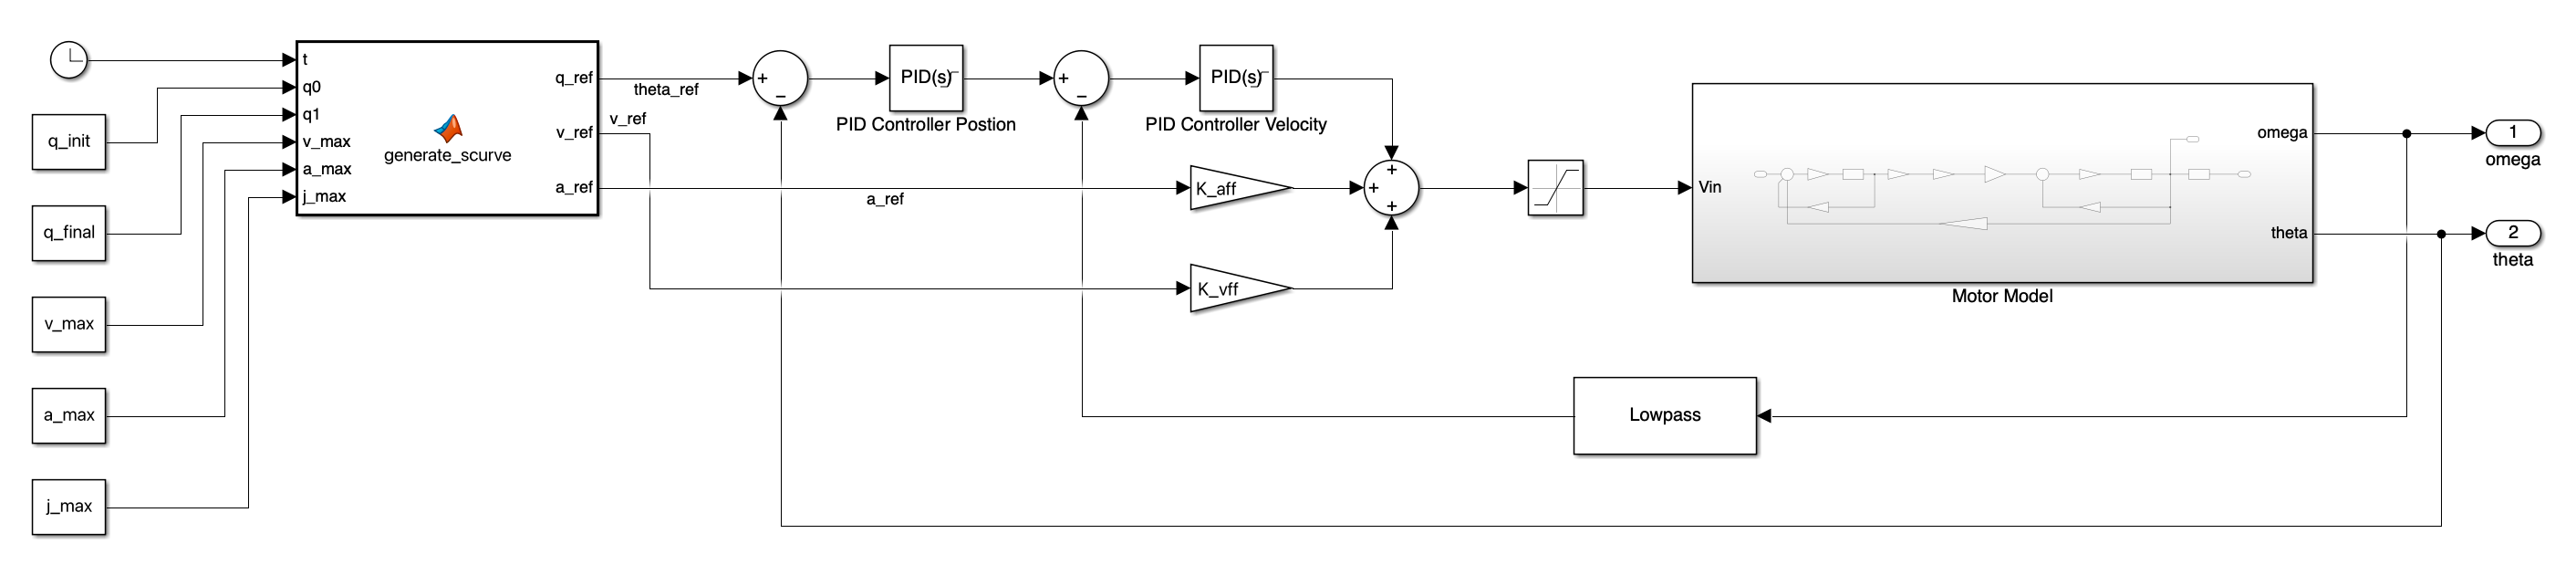
\includegraphics[width=0.95\textwidth]{images/simulink_cascade.png}
  \caption{Block Diagram ของ Cascade PID Control พร้อม Feedforward}
  \label{fig:cascade_block}
\end{figure}

\paragraph{ข้อกำหนดการออกแบบ}

\begin{table}[H]
  \centering
  \caption{ข้อกำหนดของระบบควบคุม}
  \label{tab:ctrl_req}
  \begin{tabular}{llcc}
    \toprule
    ข้อกำหนด & สัญลักษณ์ & ค่า & รหัส \\
    \midrule
    Settling Time & $t_s$  & $\leq 0.5$ s & P5 \\
    Overshoot     & $\%OS$ & $\leq 1\%$   & P6 \\
    \bottomrule
  \end{tabular}
\end{table}

\paragraph{การวิเคราะห์ Frequency Response ของ Plant}

ก่อนการออกแบบ Controller จำเป็นต้องวิเคราะห์ Frequency Response 
ของ Plant ก่อน เพื่อทำความเข้าใจพฤติกรรมของระบบในแต่ละย่านความถี่
โดยใช้ Bode Plot ซึ่งประกอบด้วยกราฟ 2 ส่วน ได้แก่

\begin{itemize}
  \item \textbf{Magnitude (dB):} แสดงอัตราส่วนขนาดระหว่าง Output และ Input 
        ที่แต่ละความถี่ เช่น $-20$\,dB หมายความว่า Output มีขนาดเล็กกว่า 
        Input อยู่ 10 เท่า ค่า 0\,dB หมายความว่า Output มีขนาดเท่ากับ Input พอดี
  \item \textbf{Phase (deg):} แสดงความล่าช้าของ Output เทียบกับ Input 
        ที่แต่ละความถี่ เช่น $-90°$ หมายความว่า Output ตามหลัง Input อยู่ 
        $\frac{1}{4}$ คาบของสัญญาณนั้น
\end{itemize}

\textbf{Velocity Plant และ Position Plant}

ระบบนี้ใช้ Plant 2 แบบขึ้นอยู่กับ Output ที่สนใจ ได้แก่

\begin{itemize}
  \item $G_{vel}(s)$: Input คือ $V_{in}$ และ Output คือ $\omega_{arm}$ 
        ใช้สำหรับออกแบบ Velocity Inner Loop
  \item $G_{pos}(s)$: Input คือ $V_{in}$ และ Output คือ $\theta_{arm}$ 
        ใช้สำหรับออกแบบ Position Outer Loop
\end{itemize}

ความสัมพันธ์ระหว่างทั้งสองคือ

\begin{equation}
  G_{pos}(s) = \frac{G_{vel}(s)}{s}
  \label{eq:gpos_gvel}
\end{equation}

การหาร $s$ เท่ากับการเพิ่ม Integrator หนึ่งตัว ส่งผลให้ Phase ของ 
$G_{pos}(s)$ ต่ำกว่า $G_{vel}(s)$ อยู่ $90°$ ตลอดทุกความถี่
ดังที่เห็นในรูปที่~\ref{fig:bode_plant} ว่า Phase ของ $G_{pos}(s)$ 
เริ่มต้นที่ $-90°$ แทนที่จะเริ่มที่ $0°$ เหมือน $G_{vel}(s)$

\textbf{การเลือก Damping Ratio $\zeta = 0.85$}

Damping Ratio $\zeta$ กำหนดจาก Overshoot Requirement ที่ระบุไว้ใน P6 
ว่า OS $\leq 1\%$ โดย Solve หาค่า $\zeta$ ขั้นต่ำที่ทำให้เงื่อนไขนี้สำเร็จ
จากสมการ Overshoot ของระบบ Second-Order

\begin{equation}
  \%OS = e^{-\pi\zeta/\sqrt{1-\zeta^2}} \times 100 \leq 1
  \label{eq:os_requirement}
\end{equation}

จัดรูปสมการโดยนำ Log ทั้งสองข้าง

\begin{equation}
  \frac{\pi\zeta}{\sqrt{1-\zeta^2}} \geq -\ln\!\left(\frac{1}{100}\right) 
  = \ln(100) = 4.605
  \label{eq:os_log}
\end{equation}

แก้สมการหา $\zeta$ ขั้นต่ำได้

\begin{equation}
  \zeta_{min} = \frac{4.605}{\sqrt{\pi^2 + 4.605^2}} 
              = \frac{4.605}{\sqrt{9.870 + 21.206}} 
              = \frac{4.605}{5.575} 
              \approx 0.826
  \label{eq:zeta_min}
\end{equation}

จึงเลือก $\zeta = 0.85$ ซึ่งสูงกว่าขีดจำกัด $\zeta_{min} = 0.826$ 
เพื่อให้มี Margin เพียงพอสำหรับความไม่แน่นอนของระบบจริง
และยืนยันได้ว่าได้ Overshoot จริงคือ

\begin{equation}
  \%OS = e^{-\pi(0.85)/\sqrt{1-0.85^2}} \times 100 
       = e^{-\pi(0.85)/0.527} \times 100 
       = 0.43\%
  \label{eq:os_verify}
\end{equation}

ซึ่งต่ำกว่าเกณฑ์ $1\%$ อย่างชัดเจน

\textbf{Phase Margin และความสำคัญต่อเสถียรภาพ}

จุดสำคัญที่ต้องอ่านจาก Bode Plot ก่อนออกแบบ Controller มีสองจุด ได้แก่

\begin{itemize}
  \item \textbf{Gain Crossover Frequency ($\omega_c$):} คือความถี่ที่ 
        Magnitude $= 0$\,dB หมายความว่าที่ความถี่นี้ Output มีขนาดเท่ากับ 
        Input พอดี $\omega_c$ บอกถึงความเร็วในการตอบสนองของระบบ 
        Closed-Loop ยิ่ง $\omega_c$ สูง ระบบยิ่งตอบสนองเร็ว
  \item \textbf{Phase Margin (PM):} คือระยะห่างระหว่าง Phase ที่ $\omega_c$ 
        กับ $-180°$ คำนวณได้จาก
        \begin{equation}
          PM = 180° + \angle G(j\omega_c)
          \label{eq:phase_margin}
        \end{equation}
        ยิ่ง PM สูง ระบบยิ่ง Stable และมี Overshoot น้อย 
        หาก PM ต่ำกว่า $0°$ ระบบจะ Oscillate ไม่หยุด
\end{itemize}

จากรูปที่~\ref{fig:bode_plant} พบว่า $G_{pos}(s)$ มีเส้นประแสดง 
$-135°$ (ซึ่งสอดคล้องกับ PM $= 45°$) และ $-180°$ ไว้เป็นเกณฑ์อ้างอิง
แสดงให้เห็นว่า Plant เปล่าๆ ยังไม่มี Phase Margin เพียงพอสำหรับ
ข้อกำหนด Overshoot $\leq 1\%$ จึงจำเป็นต้องออกแบบ Controller 
เพื่อชดเชย Phase ที่ขาดไป

\begin{figure}[H]
  \centering
  
\includegraphics[width=0.88\textwidth]{images/bode_plant.png}
  \caption{Bode Plot ของ Velocity Plant $G_{vel}(s)$ และ Position Plant $G_{pos}(s)$}
  \label{fig:bode_plant}
\end{figure}

\paragraph{การออกแบบ Velocity Inner Loop}

\textbf{ทำไมต้องเร็วกว่า Position Loop 5 เท่า}

ระบบ Cascade Control ประกอบด้วย 2 Loop ซ้อนกัน โดย Velocity Inner Loop
ทำหน้าที่ควบคุมความเร็ว และ Position Outer Loop ทำหน้าที่ควบคุมตำแหน่ง
หลักการออกแบบ Cascade Control กำหนดให้ Inner Loop ต้องตอบสนองเร็วกว่า
Outer Loop อย่างน้อย 3--10 เท่า เพื่อให้ Outer Loop มองเห็น Inner Loop
เป็นเสมือน Ideal Follower ที่ตามคำสั่งได้ทันที
หากความเร็วของทั้งสอง Loop ใกล้เคียงกัน Loop ทั้งสองจะ Interact กัน
ทำให้ระบบไม่เสถียร จึงเลือก 5 เท่าเป็นค่ากลางที่ปลอดภัย

\begin{equation}
  \omega_{c,vel} \geq 5\,\omega_{c,pos} = 5 \times 9.41 = 47.1\,\text{rad/s}
  \quad \Rightarrow \quad
  \omega_{c,vel} = 47\,\text{rad/s}
\end{equation}

\textbf{ที่มา of Phase $-82.8°$ ที่ $\omega = 47$\,rad/s}

Transfer Function ของ Velocity Plant คือ

\begin{equation}
  G_{vel}(s) = \frac{2254}{s^2 + 1003.8\,s + 8136}
\end{equation}

แทน $s = j\omega = j47$ เพื่อหา Phase

\begin{equation}
  \begin{split}
    G_{vel}(j47) &= \frac{2254}{(j47)^2 + 1003.8(j47) + 8136} \\
                 &= \frac{2254}{(8136 - 47^2) + j(1003.8 \times 47)} \\
                 &= \frac{2254}{5927 + j47{,}179}
  \end{split}
  \label{eq:gvel_j47}
\end{equation}

Phase ของ $G_{vel}(j47)$ คือ Phase ของตัวส่วน ซึ่งเป็น Complex Number

\begin{equation}
  \angle G_{vel}(j47) = -\arctan\!\left(\frac{47{,}179}{5927}\right)
                      = -\arctan(7.960)
                      = -82.8°
  \label{eq:vel_phase}
\end{equation}

หมายความว่า Plant เปล่าๆ ที่ $\omega_c = 47$\,rad/s มี Phase อยู่ที่ $-82.8°$
ดังนั้น Phase Margin ของ Plant เปล่าๆ คือ $180° - 82.8° = 97.2°$
ซึ่งสูงกว่าเกณฑ์ $70°$ แต่ยังต้องใส่ PID เพื่อปรับ Gain ให้ถูกต้อง
โดยใช้ \texttt{pidtune} ของ MATLAB ออกแบบที่ $\omega_c = 47$\,rad/s
และ $PM = 70°$ ได้ Phase Margin จริง $79.2°$

\paragraph{การออกแบบ Position Outer Loop}

การเลือก Damping Ratio $\zeta = 0.85$ และการคำนวณที่เกี่ยวข้องเป็นไปตามเกณฑ์ที่ระบุไว้ก่อนหน้าเพื่อให้ได้ Overshoot $\leq 1\%$ และ Settling Time ตามข้อกำหนด

\textbf{การคำนวณ Crossover Frequency ของ Position Loop}

กำหนด $\omega_{c,pos}$ จาก Settling Time Requirement P5 ที่ระบุว่า
$t_s \leq 0.5$\,s โดยใช้ความสัมพันธ์ของระบบ Second-Order

\begin{equation}
  t_s \approx \frac{4}{\zeta\,\omega_{c,pos}}
  \quad \Rightarrow \quad
  \omega_{c,pos} = \frac{4}{\zeta\, t_s}
                = \frac{4}{0.85 \times 0.5}
                = 9.41\,\text{rad/s}
  \label{eq:pos_target}
\end{equation}

และกำหนด $PM_{pos} \geq 80°$ เพื่อให้ได้ Damping ที่สอดคล้องกับ
$\zeta = 0.85$ ในระบบ Closed-Loop จริง
โดยใช้ความสัมพันธ์ประมาณ $PM \approx 100\zeta = 85°$
แล้วเลือก $80°$ เป็นขีดจำกัดขั้นต่ำเพื่อให้มี Margin

Open-loop Bode Plot หลัง design แสดงดัง\cref{fig:bode_openloop}

\begin{figure}[H]
  \centering
  
\includegraphics[width=0.88\textwidth]{images/bode_openloop.png}
  \caption{Open-loop Bode Plot ของ Velocity Loop และ Position Loop หลัง Design
           แสดง Crossover Frequency และ Phase Margin}
  \label{fig:bode_openloop}
\end{figure}

\paragraph{Feedforward Gains}

\textbf{ทำไมต้องมี Feedforward เพิ่มจาก PID}

PID Controller ทำงานแบบ Reactive คือรอให้เกิด Error ก่อนแล้วจึงแก้ไข
ในขณะที่ S-Curve Profile เปลี่ยน Reference ตลอดเวลา
ทำให้ PID มี Tracking Error สะสมตลอดช่วงการเคลื่อนที่
Feedforward แก้ปัญหานี้โดยคำนวณ Voltage ที่ต้องการล่วงหน้า
จาก Reference Velocity และ Acceleration โดยตรง
ทำให้ PID ต้องแก้ไขแค่ส่วนที่เหลือจาก Model Error เท่านั้น

\textbf{ที่มา of สูตร $K_{vff}$}

ที่ Steady State ความเร่งเป็นศูนย์ $\dot{\omega}_{arm} = 0$
สมการกลของระบบที่ Output Shaft คือ

\begin{equation}
  0 = \eta\, N\, K_t\, i_a - b\,\omega_{arm}
  \quad \Rightarrow \quad
  i_a = \frac{b\,\omega_{arm}}{\eta\, N\, K_t}
  \label{eq:ia_ss}
\end{equation}

แทนลงในสมการไฟฟ้าที่ Steady State ($\frac{di_a}{dt} = 0$)

\begin{equation}
  V_{in} = R_a\, i_a + K_b\, N\,\omega_{arm}
         = \frac{R_a\, b}{\eta\, N\, K_t}\,\omega_{arm} + K_b\, N\,\omega_{arm}
  \label{eq:vin_ss}
\end{equation}

ดังนั้น Velocity Feedforward Gain คือ

\begin{equation}
  \begin{split}
    K_{vff} &= \frac{V_{in}}{\omega_{arm}}
             = \frac{R_a\, b}{\eta\, N\, K_t} + K_b\, N \\
            &= \frac{1.453 \times 0.193}{0.04065 \times 0.836 \times 70}
               + 0.04165 \times 70 \\
            &= 0.118 + 2.916 = 3.034\,\text{V/(rad/s)}
  \end{split}
  \label{eq:Kvff}
\end{equation}

\textbf{ที่มา of สูตร $K_{aff}$}

ในช่วงเร่ง $\dot{\omega}_{arm} \neq 0$ สมการกลเพิ่ม Inertia Term

\begin{equation}
  J\,\dot{\omega}_{arm} = \eta\, N\, K_t\, i_a - b\,\omega_{arm}
  \quad \Rightarrow \quad
  i_a = \frac{J\,\dot{\omega}_{arm} + b\,\omega_{arm}}{\eta\, N\, K_t}
  \label{eq:ia_accel}
\end{equation}

ส่วนที่เพิ่มขึ้นเนื่องจาก Acceleration คือ

\begin{equation}
  \Delta V_{in} = R_a \cdot \frac{J\,\dot{\omega}_{arm}}{\eta\, N\, K_t}
  \label{eq:dvin_accel}
\end{equation}

ดังนั้น Acceleration Feedforward Gain คือ

\begin{equation}
  K_{aff} = \frac{\Delta V_{in}}{\dot{\omega}_{arm}}
           = \frac{R_a\, J}{\eta\, N\, K_t}
           = \frac{1.453 \times 0.728}{0.04065 \times 0.836 \times 70}
           = \frac{1.057}{2.376} = 0.445\,\text{V/(rad/s}^2\text{)}
  \label{eq:Kaff}
\end{equation}

\paragraph{Filter Coefficient $N$ และหน่วยของ PID Gains}

\textbf{Filter Coefficient $N$ คืออะไร}

Derivative Term ของ PID ในทางทฤษฎีคือ $K_d \cdot s$ ซึ่งเป็น Pure Differentiator
มีปัญหาคือขยาย Noise ความถี่สูงอย่างไม่จำกัด
ในทางปฏิบัติจึงใส่ Low-pass Filter เข้าไปใน Derivative Term ดังนี้

\begin{equation}
  D(s) = K_d \cdot \frac{N\,s}{s + N}
  \label{eq:derivative_filter}
\end{equation}

โดยที่ $N$ คือ Filter Coefficient ซึ่งกำหนด Cutoff Frequency ของ Filter
ที่ $\omega = N$\,rad/s ยิ่ง $N$ สูง Filter ตัด Noise ได้น้อยลง
แต่ Derivative ทำงานได้แม่นยำขึ้นในย่านความถี่สูง
เลือก $N_{vel} = 100$ สำหรับ Velocity Loop เพราะต้องการ Derivative
ที่ทำงานได้ถึง $\omega = 100$\,rad/s ซึ่งสูงกว่า $\omega_{c,vel} = 47$\,rad/s
และเลือก $N_{pos} = 20$ สำหรับ Position Loop เพราะ $\omega_{c,pos} = 9.41$\,rad/s
ต้องการ Derivative ที่ทำงานได้ถึง $\omega = 20$\,rad/s เท่านั้น

\paragraph{สรุปค่า PID Gains}

\begin{table}[H]
  \centering
  \caption{ค่า PID Gain ของระบบควบคุม}
  \label{tab:pid_gains}
  \begin{tabular}{llccc}
    \toprule
    Loop & Gain & สัญลักษณ์ & ค่า & หน่วย \\
    \midrule
    \multirow{4}{*}{Velocity Inner} & Proportional & $K_{p,vel}$ & 20.036  & V/(rad/s) \\
                                    & Integral     & $K_{i,vel}$ & 376.923 & V/rad \\
                                    & Derivative   & $K_{d,vel}$ & 0.0325  & V$\cdot$s/rad \\
                                    & Filter Coeff & $N_{vel}$   & 100     & -- \\
    \midrule
    \multirow{4}{*}{Position Outer} & Proportional & $K_{p,pos}$ & 9.267  & s$^{-1}$ \\
                                    & Integral     & $K_{i,pos}$ & 10.50  & s$^{-2}$ \\
                                    & Derivative   & $K_{d,pos}$ & 0.08   & s \\
                                    & Filter Coeff & $N_{pos}$   & 20     & -- \\
    \midrule
    \multirow{2}{*}{Feedforward}    & Velocity FF  & $K_{vff}$   & 3.034  & V/(rad/s) \\
                                    & Accel FF     & $K_{aff}$   & 0.445  & V/(rad/s$^2$) \\
    \bottomrule
  \end{tabular}
\end{table}

\paragraph{หมายเหตุเกี่ยวกับค่า PID Gains}

ค่า PID Gains ในตารางที่~\ref{tab:pid_gains} ได้มาจากการออกแบบด้วยวิธี 
Loop Shaping โดยใช้ \texttt{pidtune} ของ MATLAB 
และตรวจสอบสมรรถนะด้วยการ Simulate บน State Space Model 
ที่ Discretize ด้วยวิธี Zero-Order Hold (ZOH) ที่ Sampling Rate 10\,kHz
พารามิเตอร์เหล่านี้จะถูกนำไปใช้ในการประเมินสมรรถนะผ่านการ Simulation โดยผลการวิเคราะห์เปรียบเทียบกับ Requirement แสดงใน\cref{subsec:sim_results_arm}

อย่างไรก็ตาม ค่าเหล่านี้ยังเป็นค่าจากการออกแบบทางทฤษฎีบน Model เท่านั้น
ในการใช้งานจริงบน Hardware อาจจำเป็นต้องปรับ Fine-tune 
เนื่องจากปัจจัยที่ Model ไม่ได้คำนึงถึง เช่น Static Friction (Stiction) 
ของ Bearing และ Belt Drive, Backlash ของ Gearbox, Quantization Error 
ของ Encoder และ Sampling Rate จริงของ STM32 ที่ 40\,Hz

% ------------------------------------------------------------
\subsubsection{Motion Profile แบบ S-Curve}
% ------------------------------------------------------------

\paragraph{ขีดจำกัดของการเคลื่อนที่}

ขีดจำกัดของ Motion Profile คำนวณจาก Hardware Constraints ได้แก่
กระแสสูงสุด $i_{max} = 10$\,A ของ Cytron MD10C
และความเร็วสูงสุดที่วัดได้จาก Step 24\,V Test $\omega_{max} = 8.116$\,rad/s

\begin{align}
  v_{max}  &= 0.9\,\omega_{max}
            = 0.9 \times 8.116 = 7.304\,\text{rad/s}
  \label{eq:vmax}\\
  \tau_{out,max} &= K_t\,\eta\,N\,i_{max}
                 = 0.04065 \times 0.836 \times 70 \times 10
                 = 23.80\,\text{N$\cdot$m}
  \label{eq:taumax}\\
  a_{max}  &= 0.9 \times \frac{\tau_{out,max} - b\,\omega_{max}}{J}
            = 0.9 \times \frac{23.80 - 0.193 \times 8.116}{0.728}
            = 27.49\,\text{rad/s}^2
  \label{eq:amax}\\
  j_{max}  &= 0.9\,a_{max}\,\omega_{n,vel}
            = 0.9 \times 27.49 \times 56.6
            = 1400\,\text{rad/s}^3
  \label{eq:jmax}
\end{align}

\paragraph{โครงสร้าง S-Curve 7 Phase และการคำนวณ}

S-Curve Motion Profile แบ่งออกเป็น 7 Phase ดังแสดงใน\cref{tab:scurve_phases}

\begin{table}[H]
  \centering
  \caption{โครงสร้าง S-Curve 7 Phase}
  \label{tab:scurve_phases}
  \begin{tabular}{clcc}
    \toprule
    Phase & ชื่อ & Jerk & ระยะเวลา \\
    \midrule
    1 & Jerk Up (Acceleration)    & $+j_{max}$ & $t_j$ \\
    2 & Constant Acceleration     & $0$        & $t_a$ \\
    3 & Jerk Down (Acceleration)  & $-j_{max}$ & $t_j$ \\
    4 & Cruise (Constant Velocity) & $0$       & $t_v$ \\
    5 & Jerk Down (Deceleration)  & $-j_{max}$ & $t_j$ \\
    6 & Constant Deceleration     & $0$        & $t_a$ \\
    7 & Jerk Up (Deceleration)    & $+j_{max}$ & $t_j$ \\
    \bottomrule
  \end{tabular}
\end{table}

เวลาของแต่ละ Phase คำนวณจาก Motion Limits

\begin{equation}
  t_j = \frac{a_{max}}{j_{max}} = \frac{27.49}{1400} = 0.01963\,\text{s}, \qquad
  t_a = \frac{v_{max}}{a_{max}} - t_j = \frac{7.304}{27.49} - 0.01963 = 0.24607\,\text{s}
  \label{eq:tj_ta}
\end{equation}

ระยะทางช่วง Acceleration (Phase 1--3) คือ $d_{accel} = 1.042$\,rad
และเวลา Cruise คำนวณจาก

\begin{equation}
  t_v = \frac{q_{total} - 2\,d_{accel}}{v_{max}}, \qquad
  t_{move} = 4\,t_j + 2\,t_a + t_v
  \label{eq:tv_tmove}
\end{equation}

S-Curve Profile สำหรับการเคลื่อนที่ 360° แสดงดัง\cref{fig:scurve_360}

\begin{figure}[H]
  \centering
  
\includegraphics[width=0.88\textwidth]{images/scurve_360.png}
  \caption{S-Curve Motion Profile สำหรับการเคลื่อนที่ 360°
           แสดง Jerk, Acceleration, Velocity และ Position เทียบกับเวลา}
  \label{fig:scurve_360}
\end{figure}

\begin{table}[H]
  \centering
  \caption{สรุปพารามิเตอร์ Motion Profile สำหรับระยะทางต่าง ๆ}
  \label{tab:motion_summary}
  \begin{tabular}{lcccc}
    \toprule
    ระยะทาง & $q_{total}$ (rad) & $t_v$ (s) & $t_{move}$ (s) & หมายเหตุ \\
    \midrule
    90°  & $\pi/2 = 1.571$ & 0 (ไม่มี Cruise) & 0.571 & Triangle profile \\
    180° & $\pi = 3.142$   & 0.197            & 0.748 & -- \\
    360° & $2\pi = 6.283$  & 0.575            & 1.146 & Worst Case \\
    \bottomrule
  \end{tabular}
\end{table}

% ------------------------------------------------------------
\subsubsection{การ Simulation ด้วย State Space Model}
% ------------------------------------------------------------

\paragraph{State Space Model}

สร้างแบบจำลอง State Space 3 State สำหรับ Simulation
โดยเลือก State Vector $\mathbf{x} = \begin{bmatrix} i_a & \omega_{arm} & \theta_{arm} \end{bmatrix}^T$

\begin{equation}
  \dot{\mathbf{x}} = A\mathbf{x} + Bu_{in}, \qquad \mathbf{y} = C\mathbf{x}
  \label{eq:ss}
\end{equation}

\begin{equation}
  A = \begin{bmatrix}
        -R_a/L_a       & -K_b N/L_a & 0 \\
        K_t\eta N/J    & -b/J       & 0 \\
        0              & 1          & 0
      \end{bmatrix}
    = \begin{bmatrix}
        -1003.5 & -2013.0 & 0 \\
        3.265   & -0.265  & 0 \\
        0       & 1       & 0
      \end{bmatrix}
  \label{eq:A_matrix}
\end{equation}

\begin{equation}
  B = \begin{bmatrix} 1/L_a \\ 0 \\ 0 \end{bmatrix}
    = \begin{bmatrix} 690.6 \\ 0 \\ 0 \end{bmatrix}, \qquad
  C = \begin{bmatrix} 0 & 1 & 0 \\ 0 & 0 & 1 \end{bmatrix}
  \label{eq:BC_matrix}
\end{equation}

Discrete ด้วยวิธี Zero-Order Hold (ZOH) ที่ Sampling Period $T_s = 0.1$\,ms
ซึ่งน้อยกว่า Electrical Time Constant $\tau_{elec} = L_a/R_a = 1.0$\,ms อย่างน้อย 10 เท่า

\paragraph{ผลการ Simulation}

การประเมินสมรรถนะของ Cascade PID Control พร้อม S-Curve 360° กระทำผ่าน State Space Simulation เพื่อตรวจสอบการตอบสนองเชิงเวลา (Time Response) และพฤติกรรมของกระแสมอเตอร์ โดยผลการ Simulation โดยละเอียดแสดงใน\cref{subsec:sim_results_arm}

\subsection{การวิเคราะห์ผลกระทบของ Connection Rod ต่อ Cycle Time}

\subsubsection{ที่มาของปัญหา}

ในการใช้งานจริง Connection Rod จะแกว่งเมื่อแขนกลเร่งและหยุด ซึ่งอาจทำให้ไม่สามารถสวม Rod เข้ารูขนาด 14 mm ได้หากมุมแกว่งยังสูงอยู่

\subsubsection{แบบจำลอง Connection Rod}

Connection Rod มีมวล $m_{rod} = 164.08$\,g และความยาว $L_{rod} = 100$\,mm จำลองเป็น Simple Pendulum ที่ถูกกระตุ้นด้วย Angular Acceleration ของแขนกล

สมการการเคลื่อนที่ของ Rod (Linearized) คือ

\begin{equation}
  I_{pivot}\,\ddot{\phi} = -m_{rod}\,g\,l_{cm}\,\phi
                          - 2\zeta_{rod}\,\omega_{n,rod}\,I_{pivot}\,\dot{\phi}
                          - m_{rod}\,l_{cm}\,r_{arm}\,\alpha_{arm}
  \label{eq:rod_eom}
\end{equation}

ค่า Natural Frequency และ Damping Ratio ของ Rod คือ

\begin{equation}
  \omega_{n,rod} = \sqrt{\frac{m_{rod}\,g\,l_{cm}}{I_{pivot}}}
                = 12.13\,\text{rad/s}
                \quad (\,f_n = 1.93\,\text{Hz})
  \label{eq:wn_rod}
\end{equation}

\begin{equation}
  \zeta_{rod} = 0.05 \quad \Rightarrow \quad
  t_{settle,rod} \approx \frac{3}{\zeta_{rod}\,\omega_{n,rod}} \approx 4.95\,\text{s}
  \label{eq:rod_settle}
\end{equation}

\subsubsection{ข้อจำกัดด้านความแม่นยำในการ Pick และ Place}

Clearance เพียง 1\,mm ต่อข้าง ทำให้มุมแกว่งสูงสุดที่ยอมรับได้คือ

\begin{equation}
  \phi_{max} = \arcsin\!\left(\frac{1\,\text{mm}}{100\,\text{mm}}\right) \approx 0.57°
  \label{eq:phi_max}
\end{equation}

\subsubsection{การวิเคราะห์ Input Shaping และ Multi-objective Optimization}

จากการวิเคราะห์พบว่าการใช้ S-Curve Profile เพียงอย่างเดียวไม่เพียงพอในการลดการแกว่งของ Rod จึงจำเป็นต้องใช้เทคนิค Input Shaping และ NSGA-II ในการปรับพารามิเตอร์ของระบบ

\begin{equation}
  \begin{split}
    t_2 &= \frac{\pi}{\omega_{d,rod}} = \frac{\pi}{12.115} = 0.2593\,\text{s} \\
    A_1 &= \frac{1}{1+K_{ZV}} = 0.5392, \qquad
    A_2  = \frac{K_{ZV}}{1+K_{ZV}} = 0.4608
  \end{split}
  \label{eq:zv_params}
\end{equation}

การดำเนินการค้นหาค่าพารามิเตอร์ที่เหมาะสมที่สุด (Optimization) กระทำผ่านอัลกอริทึม NSGA-II เพื่อหาจุดสมดุลระหว่าง Cycle Time และ Rod Swing โดยผลการวิเคราะห์ Pareto Front และ Solution ที่เลือกแสดงใน\cref{subsec:rod_opt_results}

\subsubsection{สรุปผลและข้อจำกัดที่พบ}

ผลการวิเคราะห์แสดงให้เห็นข้อจำกัดทางกายภาพของการแก้ปัญหาด้วย Software เพียงอย่างเดียว ซึ่งนำไปสู่ข้อเสนอแนะในการปรับปรุงระบบในขั้นตอนถัดไป โดยรายละเอียดการวิเคราะห์แสดงใน\cref{subsec:rod_opt_results}
